% Options for packages loaded elsewhere
\PassOptionsToPackage{unicode}{hyperref}
\PassOptionsToPackage{hyphens}{url}
%
\documentclass[
]{article}
\usepackage{amsmath,amssymb}
\usepackage{lmodern}
\usepackage{ifxetex,ifluatex}
\ifnum 0\ifxetex 1\fi\ifluatex 1\fi=0 % if pdftex
  \usepackage[T1]{fontenc}
  \usepackage[utf8]{inputenc}
  \usepackage{textcomp} % provide euro and other symbols
\else % if luatex or xetex
  \usepackage{unicode-math}
  \defaultfontfeatures{Scale=MatchLowercase}
  \defaultfontfeatures[\rmfamily]{Ligatures=TeX,Scale=1}
\fi
% Use upquote if available, for straight quotes in verbatim environments
\IfFileExists{upquote.sty}{\usepackage{upquote}}{}
\IfFileExists{microtype.sty}{% use microtype if available
  \usepackage[]{microtype}
  \UseMicrotypeSet[protrusion]{basicmath} % disable protrusion for tt fonts
}{}
\makeatletter
\@ifundefined{KOMAClassName}{% if non-KOMA class
  \IfFileExists{parskip.sty}{%
    \usepackage{parskip}
  }{% else
    \setlength{\parindent}{0pt}
    \setlength{\parskip}{6pt plus 2pt minus 1pt}}
}{% if KOMA class
  \KOMAoptions{parskip=half}}
\makeatother
\usepackage{xcolor}
\IfFileExists{xurl.sty}{\usepackage{xurl}}{} % add URL line breaks if available
\IfFileExists{bookmark.sty}{\usepackage{bookmark}}{\usepackage{hyperref}}
\hypersetup{
  pdftitle={OBIWAN BEHAVIORAL ANALYSIS},
  pdfauthor={David Munoz Tord},
  hidelinks,
  pdfcreator={LaTeX via pandoc}}
\urlstyle{same} % disable monospaced font for URLs
\usepackage[margin=1in]{geometry}
\usepackage{color}
\usepackage{fancyvrb}
\newcommand{\VerbBar}{|}
\newcommand{\VERB}{\Verb[commandchars=\\\{\}]}
\DefineVerbatimEnvironment{Highlighting}{Verbatim}{commandchars=\\\{\}}
% Add ',fontsize=\small' for more characters per line
\usepackage{framed}
\definecolor{shadecolor}{RGB}{248,248,248}
\newenvironment{Shaded}{\begin{snugshade}}{\end{snugshade}}
\newcommand{\AlertTok}[1]{\textcolor[rgb]{0.94,0.16,0.16}{#1}}
\newcommand{\AnnotationTok}[1]{\textcolor[rgb]{0.56,0.35,0.01}{\textbf{\textit{#1}}}}
\newcommand{\AttributeTok}[1]{\textcolor[rgb]{0.77,0.63,0.00}{#1}}
\newcommand{\BaseNTok}[1]{\textcolor[rgb]{0.00,0.00,0.81}{#1}}
\newcommand{\BuiltInTok}[1]{#1}
\newcommand{\CharTok}[1]{\textcolor[rgb]{0.31,0.60,0.02}{#1}}
\newcommand{\CommentTok}[1]{\textcolor[rgb]{0.56,0.35,0.01}{\textit{#1}}}
\newcommand{\CommentVarTok}[1]{\textcolor[rgb]{0.56,0.35,0.01}{\textbf{\textit{#1}}}}
\newcommand{\ConstantTok}[1]{\textcolor[rgb]{0.00,0.00,0.00}{#1}}
\newcommand{\ControlFlowTok}[1]{\textcolor[rgb]{0.13,0.29,0.53}{\textbf{#1}}}
\newcommand{\DataTypeTok}[1]{\textcolor[rgb]{0.13,0.29,0.53}{#1}}
\newcommand{\DecValTok}[1]{\textcolor[rgb]{0.00,0.00,0.81}{#1}}
\newcommand{\DocumentationTok}[1]{\textcolor[rgb]{0.56,0.35,0.01}{\textbf{\textit{#1}}}}
\newcommand{\ErrorTok}[1]{\textcolor[rgb]{0.64,0.00,0.00}{\textbf{#1}}}
\newcommand{\ExtensionTok}[1]{#1}
\newcommand{\FloatTok}[1]{\textcolor[rgb]{0.00,0.00,0.81}{#1}}
\newcommand{\FunctionTok}[1]{\textcolor[rgb]{0.00,0.00,0.00}{#1}}
\newcommand{\ImportTok}[1]{#1}
\newcommand{\InformationTok}[1]{\textcolor[rgb]{0.56,0.35,0.01}{\textbf{\textit{#1}}}}
\newcommand{\KeywordTok}[1]{\textcolor[rgb]{0.13,0.29,0.53}{\textbf{#1}}}
\newcommand{\NormalTok}[1]{#1}
\newcommand{\OperatorTok}[1]{\textcolor[rgb]{0.81,0.36,0.00}{\textbf{#1}}}
\newcommand{\OtherTok}[1]{\textcolor[rgb]{0.56,0.35,0.01}{#1}}
\newcommand{\PreprocessorTok}[1]{\textcolor[rgb]{0.56,0.35,0.01}{\textit{#1}}}
\newcommand{\RegionMarkerTok}[1]{#1}
\newcommand{\SpecialCharTok}[1]{\textcolor[rgb]{0.00,0.00,0.00}{#1}}
\newcommand{\SpecialStringTok}[1]{\textcolor[rgb]{0.31,0.60,0.02}{#1}}
\newcommand{\StringTok}[1]{\textcolor[rgb]{0.31,0.60,0.02}{#1}}
\newcommand{\VariableTok}[1]{\textcolor[rgb]{0.00,0.00,0.00}{#1}}
\newcommand{\VerbatimStringTok}[1]{\textcolor[rgb]{0.31,0.60,0.02}{#1}}
\newcommand{\WarningTok}[1]{\textcolor[rgb]{0.56,0.35,0.01}{\textbf{\textit{#1}}}}
\usepackage{graphicx}
\makeatletter
\def\maxwidth{\ifdim\Gin@nat@width>\linewidth\linewidth\else\Gin@nat@width\fi}
\def\maxheight{\ifdim\Gin@nat@height>\textheight\textheight\else\Gin@nat@height\fi}
\makeatother
% Scale images if necessary, so that they will not overflow the page
% margins by default, and it is still possible to overwrite the defaults
% using explicit options in \includegraphics[width, height, ...]{}
\setkeys{Gin}{width=\maxwidth,height=\maxheight,keepaspectratio}
% Set default figure placement to htbp
\makeatletter
\def\fps@figure{htbp}
\makeatother
\setlength{\emergencystretch}{3em} % prevent overfull lines
\providecommand{\tightlist}{%
  \setlength{\itemsep}{0pt}\setlength{\parskip}{0pt}}
\setcounter{secnumdepth}{-\maxdimen} % remove section numbering
\usepackage{booktabs}
\usepackage{longtable}
\usepackage{array}
\usepackage{multirow}
\usepackage{wrapfig}
\usepackage{float}
\usepackage{colortbl}
\usepackage{pdflscape}
\usepackage{tabu}
\usepackage{threeparttable}
\usepackage{threeparttablex}
\usepackage[normalem]{ulem}
\usepackage{makecell}
\usepackage{xcolor}
\ifluatex
  \usepackage{selnolig}  % disable illegal ligatures
\fi

\title{OBIWAN BEHAVIORAL ANALYSIS}
\author{David Munoz Tord}
\date{}

\begin{document}
\maketitle

\hypertarget{setup}{%
\subsubsection{Setup}\label{setup}}

This file was automatically created via
\texttt{the\ Repro\ package\ (version\ 0.1.0)} using R version 4.0.1
(2020-06-06)

\begin{Shaded}
\begin{Highlighting}[]
\CommentTok{\# check\_git()}
\CommentTok{\# check\_make()}
\CommentTok{\# check\_docker()}
\end{Highlighting}
\end{Shaded}

\hypertarget{description}{%
\subsection{Description}\label{description}}

Parametric Bootstrap Test method to evaluate significance of fixed
effects in mixed-effects models (using MLE fit, nsim = 5000) and Bayes
Factor from mixed models (see Wagenmakers, 2007)

\hypertarget{demographics}{%
\subsubsection{Demographics}\label{demographics}}

\begin{Shaded}
\begin{Highlighting}[]
\FunctionTok{egltable}\NormalTok{(}\FunctionTok{c}\NormalTok{(}\StringTok{"BMI"}\NormalTok{, }\StringTok{"AGE"}\NormalTok{, }\StringTok{"GENDER"}\NormalTok{), }
  \AttributeTok{g =} \StringTok{"intervention"}\NormalTok{, }\AttributeTok{data =}\NormalTok{ df, }\AttributeTok{strict =} \ConstantTok{FALSE}\NormalTok{) }\SpecialCharTok{\%\textgreater{}\%}
  \FunctionTok{kbl}\NormalTok{(}\AttributeTok{caption =}\StringTok{"Summary statistics"}\NormalTok{, }\AttributeTok{digits =} \DecValTok{2}\NormalTok{) }\SpecialCharTok{\%\textgreater{}\%}
  \FunctionTok{kable\_styling}\NormalTok{(}\AttributeTok{latex\_options =} \StringTok{"HOLD\_position"}\NormalTok{, }\AttributeTok{position =} \StringTok{"center"}\NormalTok{, }\AttributeTok{full\_width =}\NormalTok{ F) }\SpecialCharTok{\%\textgreater{}\%}
  \FunctionTok{row\_spec}\NormalTok{(}\DecValTok{0}\NormalTok{,}\AttributeTok{bold=}\NormalTok{T,}\AttributeTok{align=}\StringTok{\textquotesingle{}c\textquotesingle{}}\NormalTok{)}
\end{Highlighting}
\end{Shaded}

\begin{table}[H]

\caption{\label{tab:demographics}Summary statistics}
\centering
\begin{tabular}[t]{l|l|l|l}
\hline
\multicolumn{1}{c}{\textbf{}} & \multicolumn{1}{c}{\textbf{Placebo M (SD)/N (\%)}} & \multicolumn{1}{c}{\textbf{Liraglutide M (SD)/N (\%)}} & \multicolumn{1}{c}{\textbf{Test}}\\
\hline
BMI & -0.20 (0.91) & 0.00 (0.90) & t(df=47) = -0.78, p = .438, d = 0.22\\
\hline
AGE & 40.27 (13.74) & 38.61 (11.72) & t(df=47) = 0.45, p = .653, d = 0.13\\
\hline
GENDER &  &  & Chi-square = 0.35, df = 1, p = .556, Phi = 0.08\\
\hline
Men & 10 (38.5) & 7 (30.4) & \\
\hline
Women & 16 (61.5) & 16 (69.6) & \\
\hline
\end{tabular}
\end{table}

\hypertarget{biomedical-data}{%
\subsubsection{Biomedical data}\label{biomedical-data}}

\hypertarget{variable-selection}{%
\paragraph{Variable Selection}\label{variable-selection}}

\begin{figure}

{\centering 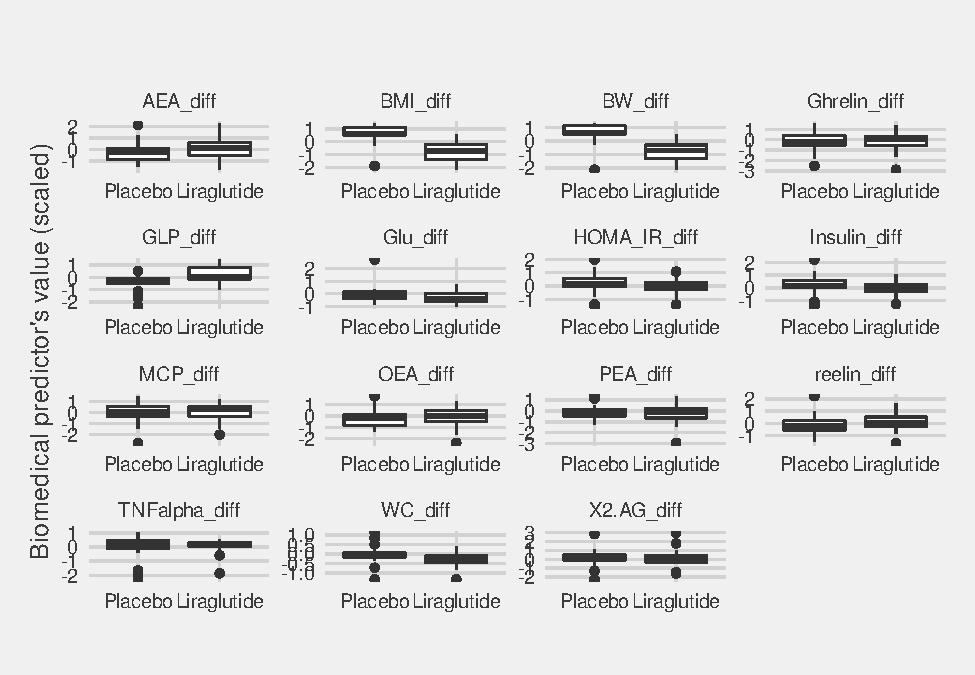
\includegraphics[width=0.9\linewidth]{OBIWAN_LIRA_files/figure-latex/var_plot-1} 

}

\caption{Box-plot of all biomedical predictors per intervention.}\label{fig:var_plot}
\end{figure}

\hfill\break
Using penalized (lasso) maximum likelihood for variable selection
(cv.glmnet), i.e.~finding the minimum lambda (regularization parameter)
to infer the best number of features to use in order to simplify the
model and avoid overfitting.\\
Using that because:\\
- Handles the problem of correlated inputs - Perform better than
stepwise selection

\begin{center}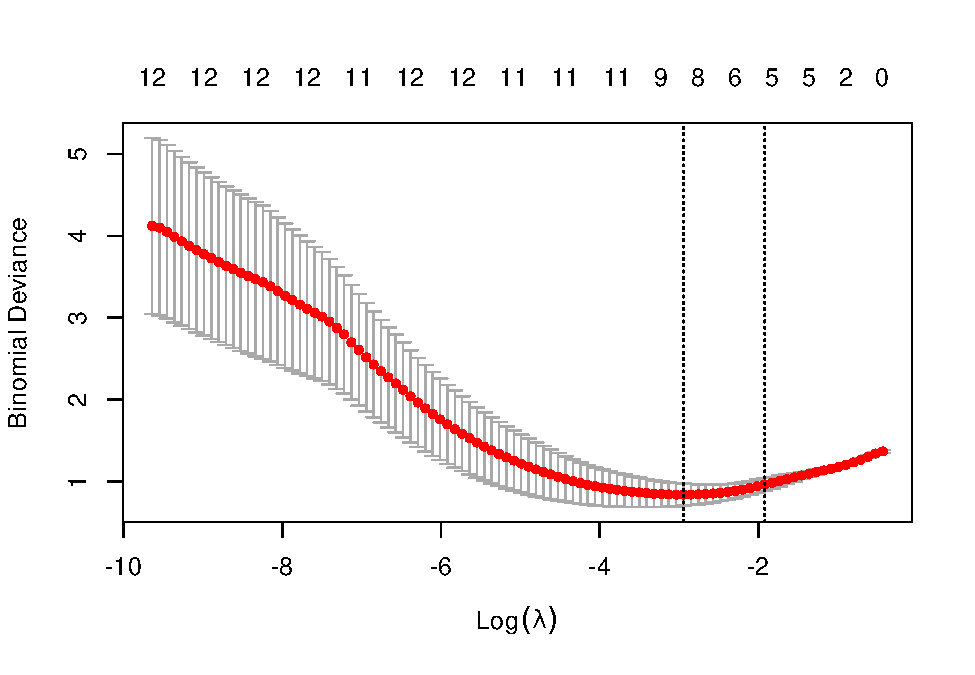
\includegraphics{OBIWAN_LIRA_files/figure-latex/var_sel-1} \end{center}

\begin{verbatim}
## [1] "BW_diff"       "BMI_diff"      "X2.AG_diff"    "reelin_diff"  
## [5] "MCP_diff"      "TNFalpha_diff" "GLP_diff"      "Glu_diff"
\end{verbatim}

\hypertarget{mediation-analysis-biomedical}{%
\paragraph{Mediation analysis
(biomedical)}\label{mediation-analysis-biomedical}}

\begin{table}[H]

\caption{\label{tab:mediate_res}Mediation Analysis: DV = Weight loss, IV = Intervention}
\centering
\begin{tabular}[t]{l|l|l|l}
\hline
 & Estimates & 95% CI & p\\
\hline
Indirect effect mediated through X2.AG_diff & -0.023 & (-0.313, 0.242) & <span> 0.848 </span>\\
\hline
Indirect effect mediated through reelin_diff & -0.105 & (-0.580, 0.270) & <span> 0.592 </span>\\
\hline
Indirect effect mediated through MCP_diff & 0.002 & (-0.199, 0.207) & <span> 0.990 </span>\\
\hline
Indirect effect mediated through TNFalpha_diff & -0.033 & (-0.271, 0.121) & <span> 0.716 </span>\\
\hline
Indirect effect mediated through GLP_diff & 0.075 & (-0.500, 0.669) & <span> 0.814 </span>\\
\hline
Indirect effect mediated through Glu_diff & -0.373 & (-0.979, 0.079) & <span> 0.112 </span>\\
\hline
Direct effect & 3.172 & (1.016, 5.485) & <span style=" font-weight: bold; " > 0.006 </span>\\
\hline
Total effect & 2.817 & (0.294, 5.471) & <span style=" font-weight: bold; " > 0.028 </span>\\
\hline
\end{tabular}
\end{table}

\hypertarget{weight-loss}{%
\subsection{Weight Loss}\label{weight-loss}}

\begin{Shaded}
\begin{Highlighting}[]
\NormalTok{res}\SpecialCharTok{$}\NormalTok{p.value }\OtherTok{=} \FunctionTok{as.numeric}\NormalTok{(res}\SpecialCharTok{$}\NormalTok{p.value)}
\NormalTok{res}\SpecialCharTok{$}\NormalTok{p.value }\OtherTok{=} \FunctionTok{ifelse}\NormalTok{(res}\SpecialCharTok{$}\NormalTok{p.value }\SpecialCharTok{\textless{}} \FloatTok{0.05}\NormalTok{,}\FunctionTok{paste}\NormalTok{(}\StringTok{"\textless{}span style=}\SpecialCharTok{\textbackslash{}"}\StringTok{ font{-}weight: bold; }\SpecialCharTok{\textbackslash{}"}\StringTok{ \textgreater{}"}\NormalTok{ ,}\FunctionTok{sprintf}\NormalTok{(}\StringTok{"\%.3f"}\NormalTok{,res}\SpecialCharTok{$}\NormalTok{p.value), }\StringTok{"\textless{}/span\textgreater{}"}\NormalTok{),  }\FunctionTok{paste}\NormalTok{(}\StringTok{"\textless{}span\textgreater{}"}\NormalTok{ ,}\FunctionTok{sprintf}\NormalTok{(}\StringTok{"\%.3f"}\NormalTok{,res}\SpecialCharTok{$}\NormalTok{p.value), }\StringTok{"\textless{}/span\textgreater{}"}\NormalTok{))}

\NormalTok{res}\SpecialCharTok{$}\NormalTok{F }\OtherTok{=} \FunctionTok{unlist}\NormalTok{(}\FunctionTok{str\_split}\NormalTok{(}\FunctionTok{gsub}\NormalTok{(}\StringTok{"[\^{}0{-}9.,{-}]"}\NormalTok{, }\StringTok{""}\NormalTok{, res}\SpecialCharTok{$}\NormalTok{F), }\StringTok{","}\NormalTok{));res}\SpecialCharTok{$}\NormalTok{pes }\OtherTok{=} \FunctionTok{unlist}\NormalTok{(}\FunctionTok{str\_split}\NormalTok{(}\FunctionTok{gsub}\NormalTok{(}\StringTok{"[\^{}0{-}9.,{-}]"}\NormalTok{, }\StringTok{""}\NormalTok{, res}\SpecialCharTok{$}\NormalTok{pes), }\StringTok{","}\NormalTok{));}
\NormalTok{res}\SpecialCharTok{$}\StringTok{\textasciigrave{}}\AttributeTok{90\% CI}\StringTok{\textasciigrave{}} \OtherTok{=} \FunctionTok{paste}\NormalTok{(}\FunctionTok{sprintf}\NormalTok{(}\StringTok{"\%.3f"}\NormalTok{,PES.weight[,}\DecValTok{2}\NormalTok{]), }\StringTok{"{-}"}\NormalTok{, }\FunctionTok{sprintf}\NormalTok{(}\StringTok{"\%.3f"}\NormalTok{,PES.weight[,}\DecValTok{3}\NormalTok{]))}

\NormalTok{res}\SpecialCharTok{$}\NormalTok{p.value[}\DecValTok{1}\NormalTok{]}\OtherTok{=} \StringTok{"\textless{}span style=}\SpecialCharTok{\textbackslash{}"}\StringTok{ font{-}weight: bold;    }\SpecialCharTok{\textbackslash{}"}\StringTok{ \textgreater{}\textbackslash{}u003C 0.001\textless{}/span\textgreater{}"}
\NormalTok{res}\SpecialCharTok{$}\NormalTok{pes[}\DecValTok{4}\NormalTok{]}\OtherTok{=} \StringTok{"\textbackslash{}u003C 0.001"}
\FunctionTok{colnames}\NormalTok{(res)[}\DecValTok{3}\SpecialCharTok{:}\DecValTok{5}\NormalTok{] }\OtherTok{=} \FunctionTok{c}\NormalTok{( }\FunctionTok{paste}\NormalTok{(}\StringTok{"F("}\NormalTok{, res}\SpecialCharTok{$}\NormalTok{df[}\DecValTok{1}\NormalTok{], }\StringTok{")"}\NormalTok{, }\AttributeTok{sep=}\StringTok{""}\NormalTok{),}\StringTok{"\&eta;\textless{}sub\textgreater{}p\textless{}/sub\textgreater{}\textless{}sup\textgreater{}2\textless{}/sup\textgreater{}"}\NormalTok{, }\StringTok{"p"}\NormalTok{)}
\NormalTok{res[}\FunctionTok{c}\NormalTok{(}\DecValTok{1}\NormalTok{,}\DecValTok{4}\NormalTok{,}\DecValTok{6}\NormalTok{,}\DecValTok{3}\NormalTok{,}\DecValTok{5}\NormalTok{)]  }\SpecialCharTok{\%\textgreater{}\%} \FunctionTok{kbl}\NormalTok{(}\AttributeTok{digits =} \DecValTok{2}\NormalTok{, }\AttributeTok{escape =}\NormalTok{ F) }\SpecialCharTok{\%\textgreater{}\%}
  \FunctionTok{kable\_styling}\NormalTok{(}\AttributeTok{latex\_options =} \StringTok{"striped"}\NormalTok{, }\AttributeTok{position =} \StringTok{"center"}\NormalTok{, }\AttributeTok{full\_width =}\NormalTok{ F) }
\end{Highlighting}
\end{Shaded}

\begin{table}[H]
\centering
\begin{tabular}[t]{l|l|l|l|l}
\hline
Effect & &eta;<sub>p</sub><sup>2</sup> & 90% CI & F(1, 42) & p\\
\hline
\cellcolor{gray!6}{intervention} & \cellcolor{gray!6}{.506} & \cellcolor{gray!6}{0.316 - 0.624} & \cellcolor{gray!6}{43.00} & \cellcolor{gray!6}{<span style=" font-weight: bold;    " >< 0.001</span>}\\
\hline
gender & .011 & 0.000 - 0.108 & 0.46 & <span> 0.500 </span>\\
\hline
\cellcolor{gray!6}{age} & \cellcolor{gray!6}{.095} & \cellcolor{gray!6}{0.002 - 0.245} & \cellcolor{gray!6}{4.41} & \cellcolor{gray!6}{<span style=" font-weight: bold; " > 0.042 </span>}\\
\hline
Date_diff & < 0.001 & 0.000 - NA & 0.00 & <span> 0.971 </span>\\
\hline
\end{tabular}
\end{table}

\begin{Shaded}
\begin{Highlighting}[]
\CommentTok{\#print(\textquotesingle{}PES: intervention: Overall higher weight loss for treament (Liraglutide) group\textquotesingle{})}
\CommentTok{\#PES.weight[1,]}
\end{Highlighting}
\end{Shaded}

\begin{figure}

{\centering 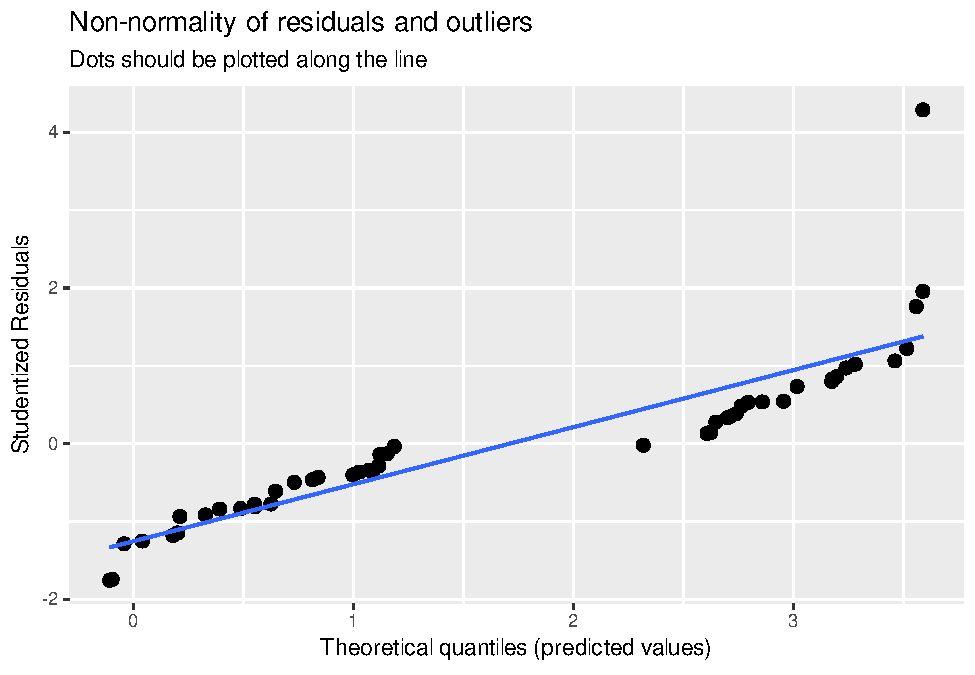
\includegraphics[width=0.25\linewidth]{OBIWAN_LIRA_files/figure-latex/unnamed-chunk-2-1} 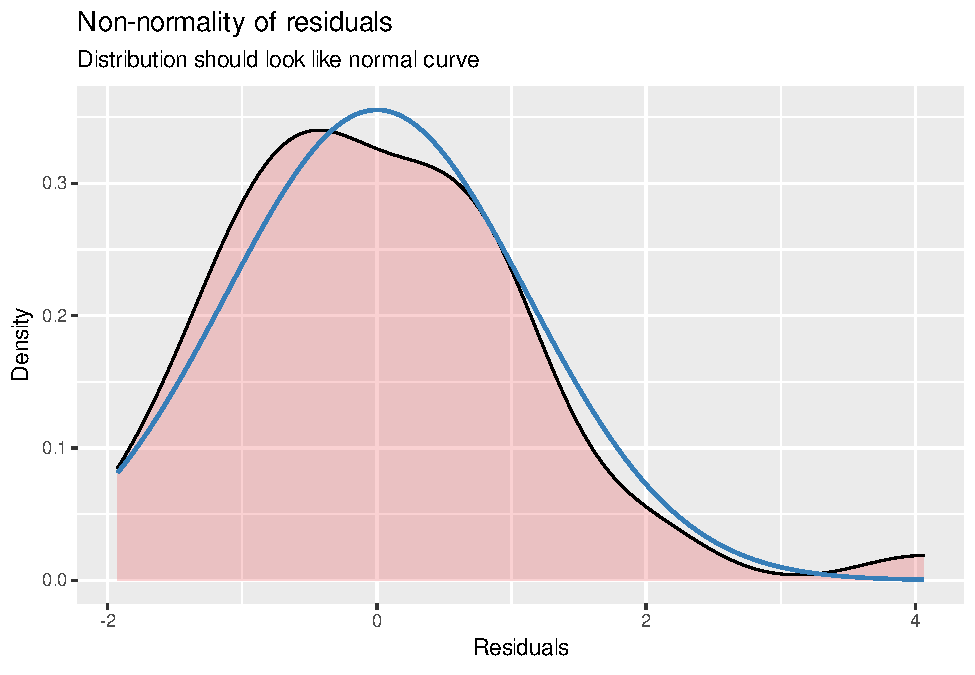
\includegraphics[width=0.25\linewidth]{OBIWAN_LIRA_files/figure-latex/unnamed-chunk-2-2} 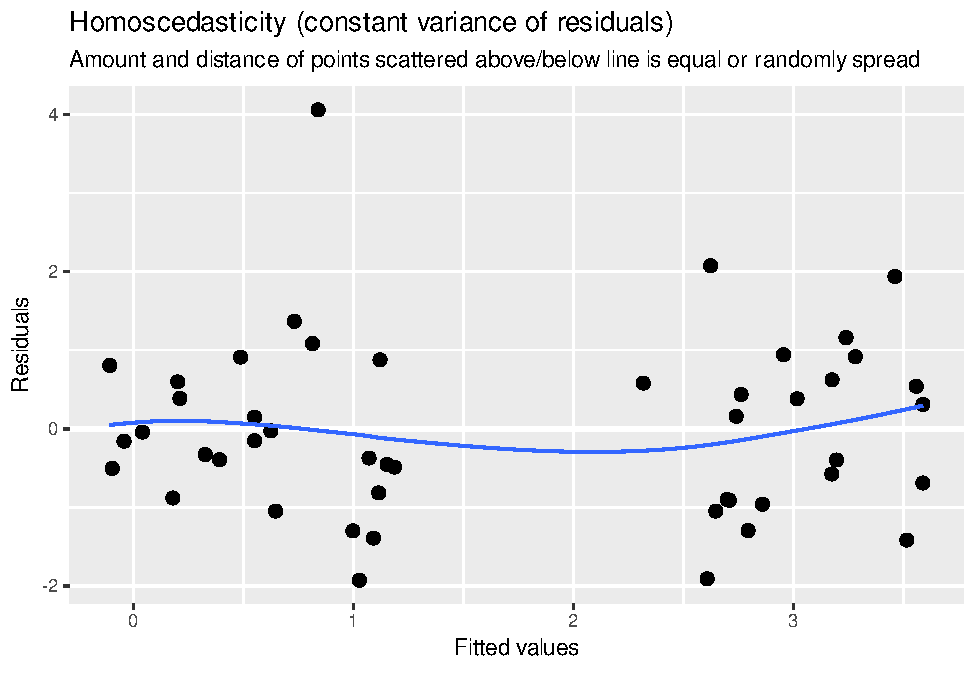
\includegraphics[width=0.25\linewidth]{OBIWAN_LIRA_files/figure-latex/unnamed-chunk-2-3} 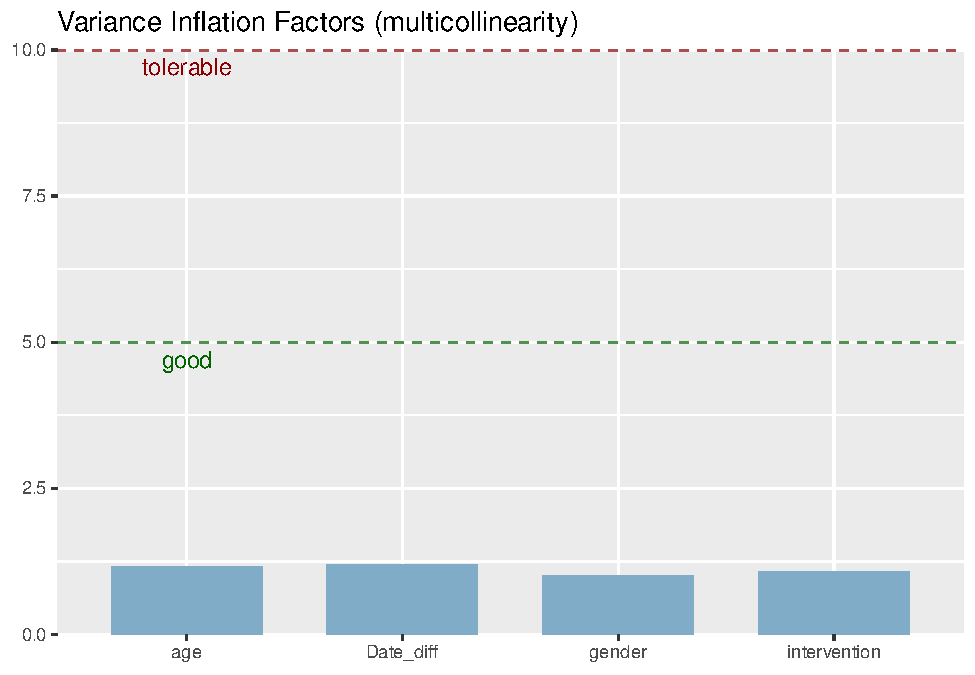
\includegraphics[width=0.25\linewidth]{OBIWAN_LIRA_files/figure-latex/unnamed-chunk-2-4} 

}

\caption{Model assumptions.}\label{fig:unnamed-chunk-2}
\end{figure}

\begin{figure}

{\centering 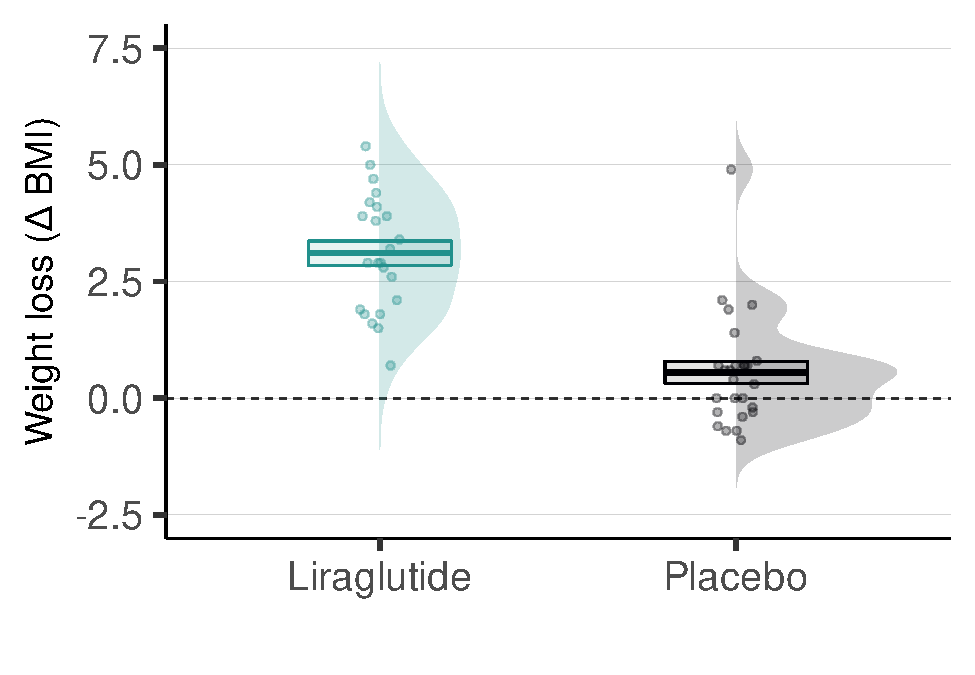
\includegraphics{OBIWAN_LIRA_files/figure-latex/Weight_Loss-1} 

}

\caption{Weight Loss by intervention.}\label{fig:Weight_Loss}
\end{figure}

\hfill\break
\hfill\break

\hypertarget{pavlvovian-conditioning-task-latency}{%
\subsection{Pavlvovian Conditioning Task
(Latency)}\label{pavlvovian-conditioning-task-latency}}

Latency = time to detect the target (ms) \& condition = CS+ or CS-\\

\hfill\break

\begin{Shaded}
\begin{Highlighting}[]
\NormalTok{tables }\OtherTok{\textless{}{-}} \FunctionTok{list.clean}\NormalTok{(}\FunctionTok{readHTMLTable}\NormalTok{(}\StringTok{"tmp/temp1.html"}\NormalTok{), }\AttributeTok{fun =}\NormalTok{ is.null, }\AttributeTok{recursive =} \ConstantTok{FALSE}\NormalTok{)}
\NormalTok{tables2 }\OtherTok{=}\NormalTok{ tables[[}\DecValTok{1}\NormalTok{]] }\SpecialCharTok{\%\textgreater{}\%}\NormalTok{ janitor}\SpecialCharTok{::}\FunctionTok{row\_to\_names}\NormalTok{(}\AttributeTok{row\_number =} \DecValTok{1}\NormalTok{)}

\NormalTok{tables2 }\OtherTok{\textless{}{-}} \FunctionTok{as.matrix}\NormalTok{(tables2) }\SpecialCharTok{\%\textgreater{}\%} \FunctionTok{as\_tibble}\NormalTok{()}
\NormalTok{tables2[}\FunctionTok{is.na}\NormalTok{(tables2)] }\OtherTok{\textless{}{-}} \StringTok{""}
\NormalTok{tables3 }\OtherTok{=}\NormalTok{ tables2[}\DecValTok{1}\SpecialCharTok{:}\FunctionTok{length}\NormalTok{(table}\SpecialCharTok{$}\NormalTok{Effect),}\DecValTok{1}\SpecialCharTok{:}\DecValTok{4}\NormalTok{] }
\NormalTok{tables3[}\DecValTok{5}\NormalTok{] }\OtherTok{=} \FunctionTok{str\_split}\NormalTok{(}\FunctionTok{gsub}\NormalTok{(}\StringTok{"[\^{}0{-}9.,{-}]"}\NormalTok{, }\StringTok{""}\NormalTok{, table[}\DecValTok{3}\NormalTok{]), }\StringTok{","}\NormalTok{)[[}\DecValTok{1}\NormalTok{]]; tables3[}\DecValTok{6}\NormalTok{] }\OtherTok{=} \FunctionTok{as.numeric}\NormalTok{(}\FunctionTok{str\_split}\NormalTok{(}\FunctionTok{gsub}\NormalTok{(}\StringTok{"[\^{}0{-}9.,{-}]"}\NormalTok{, }\StringTok{""}\NormalTok{, table[}\DecValTok{4}\NormalTok{]), }\StringTok{","}\NormalTok{)[[}\DecValTok{1}\NormalTok{]]); }
\NormalTok{tables3}\SpecialCharTok{$}\NormalTok{...}\DecValTok{6} \OtherTok{=} \FunctionTok{ifelse}\NormalTok{(tables3}\SpecialCharTok{$}\NormalTok{...}\DecValTok{6} \SpecialCharTok{\textless{}} \FloatTok{0.05}\NormalTok{,}\FunctionTok{paste}\NormalTok{(}\StringTok{"\textless{}span style=}\SpecialCharTok{\textbackslash{}"}\StringTok{ font{-}weight: bold; }\SpecialCharTok{\textbackslash{}"}\StringTok{ \textgreater{}"}\NormalTok{ ,}\FunctionTok{sprintf}\NormalTok{(}\StringTok{"\%.3f"}\NormalTok{,tables3}\SpecialCharTok{$}\NormalTok{...}\DecValTok{6}\NormalTok{), }\StringTok{"\textless{}/span\textgreater{}"}\NormalTok{),  }\FunctionTok{paste}\NormalTok{(}\StringTok{"\textless{}span\textgreater{}"}\NormalTok{ ,}\FunctionTok{sprintf}\NormalTok{(}\StringTok{"\%.3f"}\NormalTok{,tables3}\SpecialCharTok{$}\NormalTok{...}\DecValTok{6}\NormalTok{), }\StringTok{"\textless{}/span\textgreater{}"}\NormalTok{))}
\FunctionTok{colnames}\NormalTok{(tables3)[}\DecValTok{5}\NormalTok{] }\OtherTok{=} \StringTok{"\textbackslash{}u03C7\textbackslash{}u00B2"}\NormalTok{; }\FunctionTok{colnames}\NormalTok{(tables3)[}\DecValTok{6}\NormalTok{] }\OtherTok{=} \StringTok{"p"}
\NormalTok{tables3}\SpecialCharTok{$}\NormalTok{p[}\DecValTok{1}\NormalTok{]}\OtherTok{=} \StringTok{"\textless{}span style=}\SpecialCharTok{\textbackslash{}"}\StringTok{ font{-}weight: bold;    }\SpecialCharTok{\textbackslash{}"}\StringTok{ \textgreater{}\textbackslash{}u003C 0.001\textless{}/span\textgreater{}"}
\NormalTok{tables3 }\SpecialCharTok{\%\textgreater{}\%}   
  \FunctionTok{kbl}\NormalTok{(}\AttributeTok{caption =}\StringTok{"Latency (ms)"}\NormalTok{,}\AttributeTok{escape =}\NormalTok{ F) }\SpecialCharTok{\%\textgreater{}\%}
  \FunctionTok{kable\_styling}\NormalTok{(}\AttributeTok{latex\_options =} \StringTok{"HOLD\_position"}\NormalTok{, }\AttributeTok{position =} \StringTok{"center"}\NormalTok{, }\AttributeTok{full\_width =}\NormalTok{ F) }\SpecialCharTok{\%\textgreater{}\%}  \FunctionTok{row\_spec}\NormalTok{(}\DecValTok{0}\NormalTok{,}\AttributeTok{bold=}\NormalTok{T,}\AttributeTok{align=}\StringTok{\textquotesingle{}c\textquotesingle{}}\NormalTok{)}
\end{Highlighting}
\end{Shaded}

\begin{table}[H]

\caption{\label{tab:PAV_RT_mod}Latency (ms)}
\centering
\begin{tabular}[t]{l|l|l|l|l|l}
\hline
\multicolumn{1}{c}{\textbf{Predictors}} & \multicolumn{1}{c}{\textbf{Estimates}} & \multicolumn{1}{c}{\textbf{std. Error}} & \multicolumn{1}{c}{\textbf{CI}} & \multicolumn{1}{c}{\textbf{χ²}} & \multicolumn{1}{c}{\textbf{p}}\\
\hline
condition [1] & 13.39 & 2.93 & 7.65 – 19.14 & 17.69 & <span style=" font-weight: bold;    " >< 0.001</span>\\
\hline
intervention [1] & -16.75 & 12.75 & -41.74 – 8.23 & 1.64 & <span> 0.200 </span>\\
\hline
session [1] & -7.76 & 8.42 & -24.26 – 8.75 & 0.84 & <span> 0.358 </span>\\
\hline
age & 30.28 & 11.83 & 7.09 – 53.47 & 5.74 & <span style=" font-weight: bold; " > 0.017 </span>\\
\hline
gender [1] & -6.94 & 12.14 & -30.74 – 16.85 & 0.32 & <span> 0.574 </span>\\
\hline
BMI_V1 & -14.63 & 11.90 & -37.96 – 8.69 & 1.37 & <span> 0.241 </span>\\
\hline
thirsty & 28.66 & 11.39 & 6.33 – 50.99 & 5.51 & <span style=" font-weight: bold; " > 0.019 </span>\\
\hline
hungry & -20.10 & 11.41 & -42.45 – 2.25 & 3.01 & <span> 0.083 </span>\\
\hline
condition [1] *intervention [1] & -1.00 & 2.94 & -6.76 – 4.75 & 0.11 & <span> 0.735 </span>\\
\hline
condition [1] * session[1] & -4.07 & 2.72 & -9.40 – 1.25 & 2.16 & <span> 0.141 </span>\\
\hline
intervention [1] *session [1] & -11.75 & 8.38 & -28.17 – 4.68 & 1.89 & <span> 0.170 </span>\\
\hline
condition [1] * age & -5.41 & 2.64 & -10.58 – -0.25 & 3.97 & <span style=" font-weight: bold; " > 0.046 </span>\\
\hline
(condition [1] *intervention [1]) *session [1] & -2.08 & 2.72 & -7.40 – 3.24 & 0.58 & <span> 0.448 </span>\\
\hline
\end{tabular}
\end{table}

\begin{Shaded}
\begin{Highlighting}[]
\NormalTok{tmp }\OtherTok{=}\NormalTok{ tables2[(}\FunctionTok{length}\NormalTok{(table}\SpecialCharTok{$}\NormalTok{Effect)}\SpecialCharTok{+}\DecValTok{1}\NormalTok{)}\SpecialCharTok{:}\NormalTok{(}\FunctionTok{length}\NormalTok{(table}\SpecialCharTok{$}\NormalTok{Effect)}\SpecialCharTok{+}\DecValTok{5}\NormalTok{),}\DecValTok{1}\SpecialCharTok{:}\DecValTok{2}\NormalTok{]}
\FunctionTok{names}\NormalTok{(tmp) }\OtherTok{\textless{}{-}} \ConstantTok{NULL}
\NormalTok{tmp1 }\OtherTok{\textless{}{-}} \FunctionTok{data.frame}\NormalTok{(}\FunctionTok{t}\NormalTok{(tmp[}\SpecialCharTok{{-}}\DecValTok{1}\NormalTok{]))}
\FunctionTok{colnames}\NormalTok{(tmp1) }\OtherTok{\textless{}{-}}\NormalTok{ tmp[[}\DecValTok{1}\NormalTok{]]}
\NormalTok{tmp1 }\SpecialCharTok{\%\textgreater{}\%} \FunctionTok{kbl}\NormalTok{(}\AttributeTok{digits =} \DecValTok{2}\NormalTok{) }\SpecialCharTok{\%\textgreater{}\%}
  \FunctionTok{kable\_styling}\NormalTok{(}\AttributeTok{latex\_options =} \StringTok{"HOLD\_position"}\NormalTok{, }\AttributeTok{position =} \StringTok{"center"}\NormalTok{, }\AttributeTok{full\_width =}\NormalTok{ F) }
\end{Highlighting}
\end{Shaded}

\begin{table}[H]
\centering
\begin{tabular}[t]{l|l|l|l|l}
\hline
ICC & N id & N trialxcondition & Observations & Marginal R2 / Conditional R2\\
\hline
0.43 & 64 & 20 & 3888 & 0.067 / 0.472\\
\hline
\end{tabular}
\end{table}

\hfill\break

\begin{figure}

{\centering 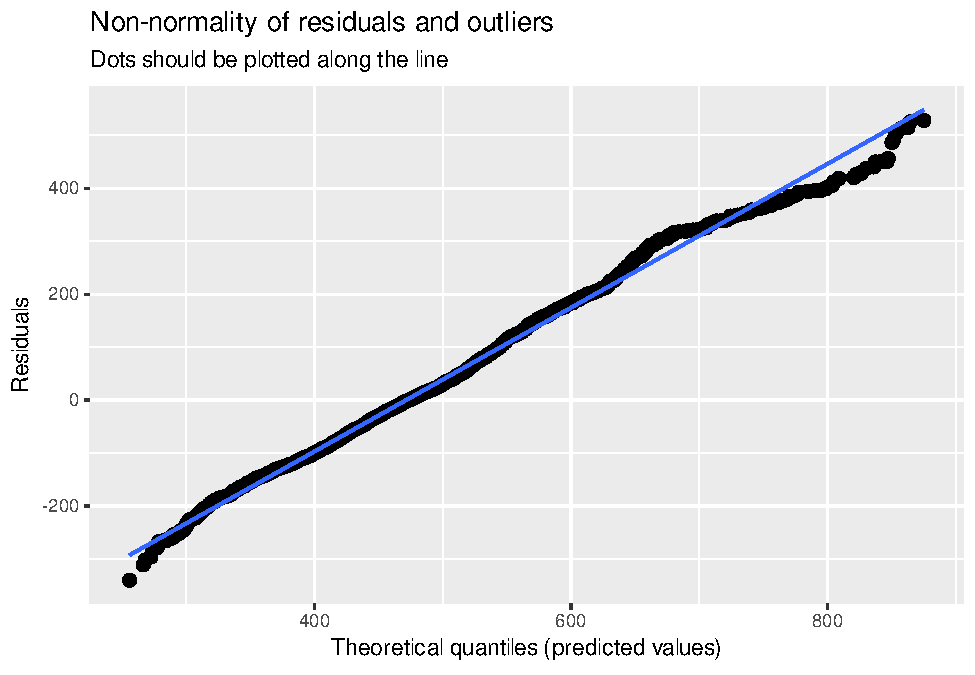
\includegraphics[width=0.25\linewidth]{OBIWAN_LIRA_files/figure-latex/unnamed-chunk-3-1} 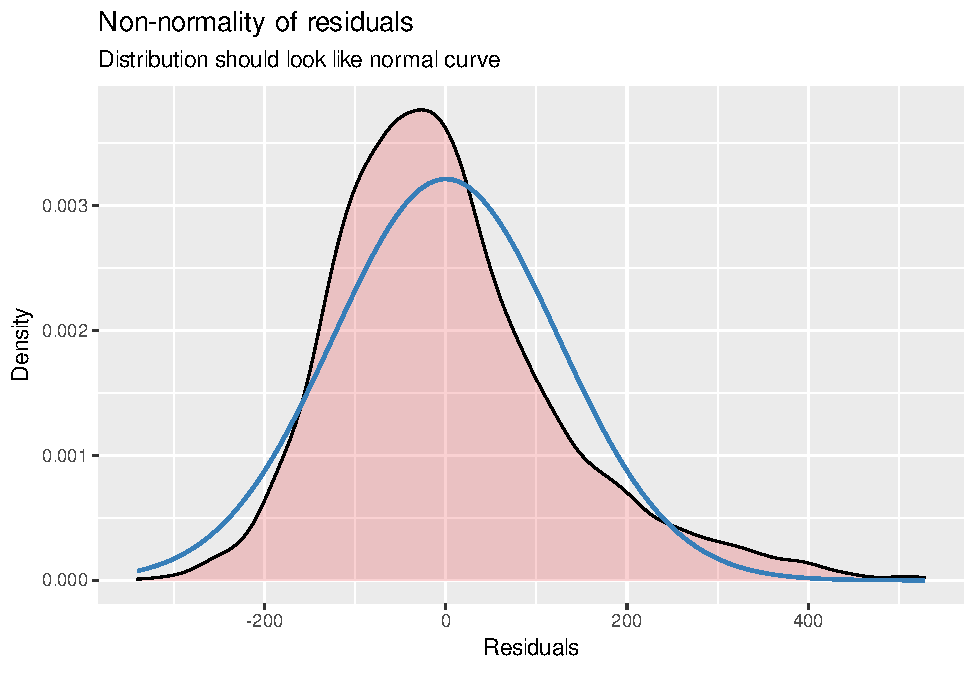
\includegraphics[width=0.25\linewidth]{OBIWAN_LIRA_files/figure-latex/unnamed-chunk-3-2} 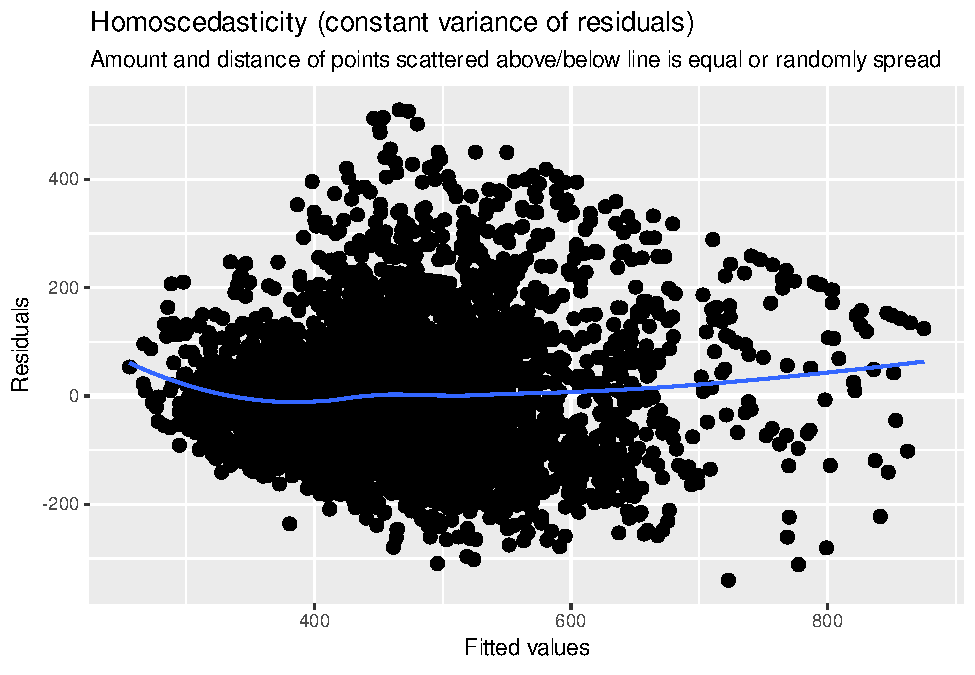
\includegraphics[width=0.25\linewidth]{OBIWAN_LIRA_files/figure-latex/unnamed-chunk-3-3} 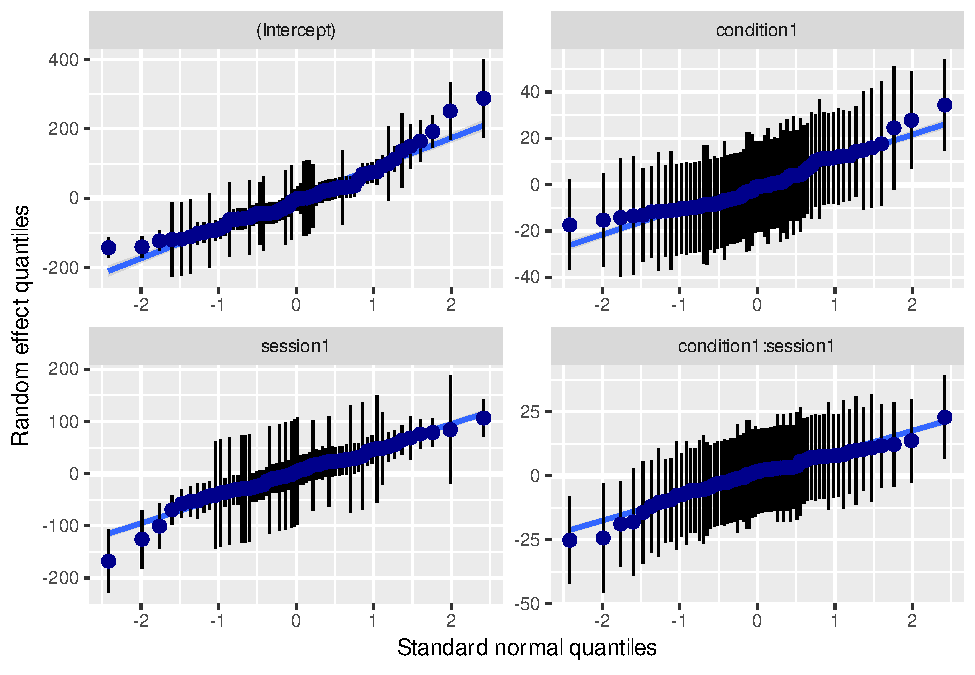
\includegraphics[width=0.25\linewidth]{OBIWAN_LIRA_files/figure-latex/unnamed-chunk-3-4} 

}

\caption{Model assumptions.}\label{fig:unnamed-chunk-3}
\end{figure}

\hfill\break
\hfill\break

\begin{figure}

{\centering 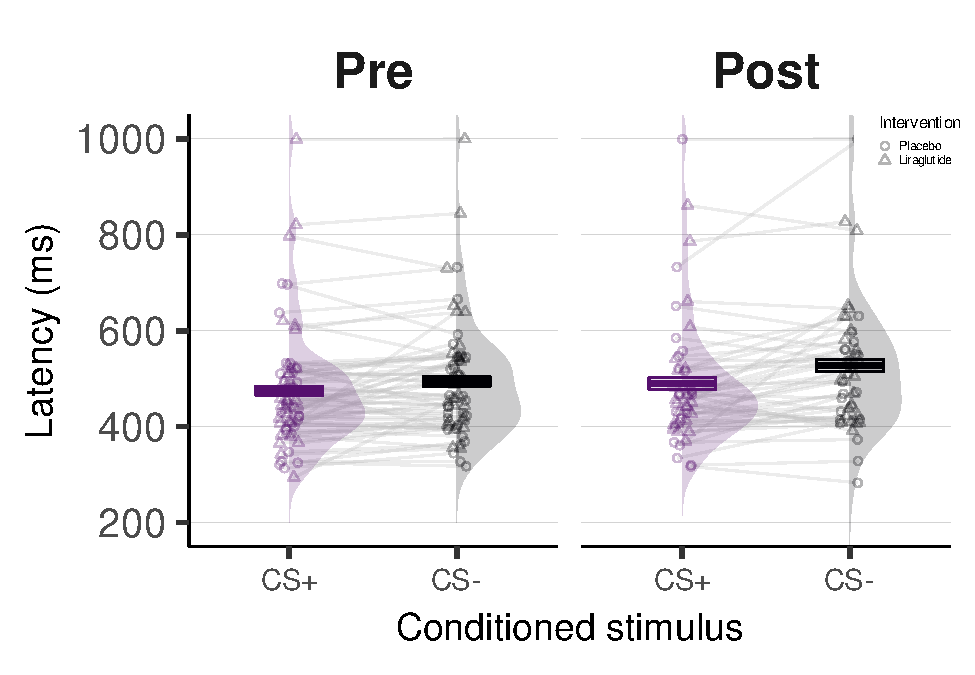
\includegraphics{OBIWAN_LIRA_files/figure-latex/PAV_RT_plot-1} 

}

\caption{Latency by pavlvovian cue.}\label{fig:PAV_RT_plot}
\end{figure}

\hypertarget{part-2-pavlvovian-conditioning-task-pleasantness-ratings}{%
\subsubsection{(Part 2) Pavlvovian Conditioning Task (Pleasantness
Ratings)}\label{part-2-pavlvovian-conditioning-task-pleasantness-ratings}}

Ratings = how pleasant is the clue (0-100, no repetitions) \& condition
= CS+ or CS-

\begin{Shaded}
\begin{Highlighting}[]
\NormalTok{res}\SpecialCharTok{$}\NormalTok{p.value }\OtherTok{=} \FunctionTok{as.numeric}\NormalTok{(res}\SpecialCharTok{$}\NormalTok{p.value)}
\NormalTok{res}\SpecialCharTok{$}\NormalTok{p.value }\OtherTok{=} \FunctionTok{ifelse}\NormalTok{(res}\SpecialCharTok{$}\NormalTok{p.value }\SpecialCharTok{\textless{}} \FloatTok{0.05}\NormalTok{,}\FunctionTok{paste}\NormalTok{(}\StringTok{"\textless{}span style=}\SpecialCharTok{\textbackslash{}"}\StringTok{ font{-}weight: bold; }\SpecialCharTok{\textbackslash{}"}\StringTok{ \textgreater{}"}\NormalTok{ ,}\FunctionTok{sprintf}\NormalTok{(}\StringTok{"\%.3f"}\NormalTok{,res}\SpecialCharTok{$}\NormalTok{p.value), }\StringTok{"\textless{}/span\textgreater{}"}\NormalTok{),  }\FunctionTok{paste}\NormalTok{(}\StringTok{"\textless{}span\textgreater{}"}\NormalTok{ ,}\FunctionTok{sprintf}\NormalTok{(}\StringTok{"\%.3f"}\NormalTok{,res}\SpecialCharTok{$}\NormalTok{p.value), }\StringTok{"\textless{}/span\textgreater{}"}\NormalTok{))}

\NormalTok{res}\SpecialCharTok{$}\NormalTok{F }\OtherTok{=} \FunctionTok{unlist}\NormalTok{(}\FunctionTok{str\_split}\NormalTok{(}\FunctionTok{gsub}\NormalTok{(}\StringTok{"[\^{}0{-}9.,{-}]"}\NormalTok{, }\StringTok{""}\NormalTok{, res}\SpecialCharTok{$}\NormalTok{F), }\StringTok{","}\NormalTok{));res}\SpecialCharTok{$}\NormalTok{pes }\OtherTok{=} \FunctionTok{unlist}\NormalTok{(}\FunctionTok{str\_split}\NormalTok{(}\FunctionTok{gsub}\NormalTok{(}\StringTok{"[\^{}0{-}9.,{-}]"}\NormalTok{, }\StringTok{""}\NormalTok{, res}\SpecialCharTok{$}\NormalTok{pes), }\StringTok{","}\NormalTok{));}
\NormalTok{res}\SpecialCharTok{$}\StringTok{\textasciigrave{}}\AttributeTok{90\% CI}\StringTok{\textasciigrave{}} \OtherTok{=} \FunctionTok{paste}\NormalTok{(}\FunctionTok{sprintf}\NormalTok{(}\StringTok{"\%.3f"}\NormalTok{,PES.lik[,}\DecValTok{2}\NormalTok{]), }\StringTok{"{-}"}\NormalTok{, }\FunctionTok{sprintf}\NormalTok{(}\StringTok{"\%.3f"}\NormalTok{,PES.lik[,}\DecValTok{3}\NormalTok{]))}

\NormalTok{res}\SpecialCharTok{$}\NormalTok{p.value[}\DecValTok{1}\NormalTok{]}\OtherTok{=} \StringTok{"\textless{}span style=}\SpecialCharTok{\textbackslash{}"}\StringTok{ font{-}weight: bold;    }\SpecialCharTok{\textbackslash{}"}\StringTok{ \textgreater{}\textbackslash{}u003C 0.001\textless{}/span\textgreater{}"}
\NormalTok{res}\SpecialCharTok{$}\NormalTok{pes[}\FunctionTok{c}\NormalTok{(}\DecValTok{5}\NormalTok{,}\DecValTok{7}\NormalTok{,}\DecValTok{8}\NormalTok{)]}\OtherTok{=} \FunctionTok{c}\NormalTok{(}\StringTok{"\textbackslash{}u003C 0.001"}\NormalTok{)}
\FunctionTok{colnames}\NormalTok{(res)[}\DecValTok{3}\SpecialCharTok{:}\DecValTok{5}\NormalTok{] }\OtherTok{=} \FunctionTok{c}\NormalTok{( }\FunctionTok{paste}\NormalTok{(}\StringTok{"F("}\NormalTok{, res}\SpecialCharTok{$}\NormalTok{df[}\DecValTok{1}\NormalTok{], }\StringTok{")"}\NormalTok{, }\AttributeTok{sep=}\StringTok{""}\NormalTok{),}\StringTok{"\&eta;\textless{}sub\textgreater{}p\textless{}/sub\textgreater{}\textless{}sup\textgreater{}2\textless{}/sup\textgreater{}"}\NormalTok{, }\StringTok{"p"}\NormalTok{)}
\NormalTok{res[}\FunctionTok{c}\NormalTok{(}\DecValTok{1}\NormalTok{,}\DecValTok{4}\NormalTok{,}\DecValTok{6}\NormalTok{,}\DecValTok{3}\NormalTok{,}\DecValTok{5}\NormalTok{)]  }\SpecialCharTok{\%\textgreater{}\%} \FunctionTok{kbl}\NormalTok{(}\AttributeTok{digits =} \DecValTok{2}\NormalTok{, }\AttributeTok{escape =}\NormalTok{ F,}\AttributeTok{row.names =}\NormalTok{ F)  }\SpecialCharTok{\%\textgreater{}\%}
  \FunctionTok{kable\_styling}\NormalTok{(}\AttributeTok{latex\_options =} \StringTok{"striped"}\NormalTok{, }\AttributeTok{position =} \StringTok{"center"}\NormalTok{, }\AttributeTok{full\_width =}\NormalTok{ F) }
\end{Highlighting}
\end{Shaded}

\begin{table}[H]
\centering
\begin{tabular}[t]{l|l|l|l|l}
\hline
Effect & &eta;<sub>p</sub><sup>2</sup> & 90% CI & F(1, 43) & p\\
\hline
\cellcolor{gray!6}{condition} & \cellcolor{gray!6}{.284} & \cellcolor{gray!6}{0.154 - 0.488} & \cellcolor{gray!6}{17.05} & \cellcolor{gray!6}{<span style=" font-weight: bold;    " >< 0.001</span>}\\
\hline
intervention & .069 & 0.000 - 0.210 & 3.21 & <span> 0.080 </span>\\
\hline
\cellcolor{gray!6}{age} & \cellcolor{gray!6}{.005} & \cellcolor{gray!6}{0.000 - 0.086} & \cellcolor{gray!6}{0.22} & \cellcolor{gray!6}{<span> 0.644 </span>}\\
\hline
gender & .054 & 0.000 - 0.188 & 2.48 & <span> 0.123 </span>\\
\hline
\cellcolor{gray!6}{BMI_V1} & \cellcolor{gray!6}{< 0.001} & \cellcolor{gray!6}{0.000 - 0.044} & \cellcolor{gray!6}{0.03} & \cellcolor{gray!6}{<span> 0.862 </span>}\\
\hline
session & .064 & 0.000 - 0.233 & 2.93 & <span> 0.094 </span>\\
\hline
\cellcolor{gray!6}{intervention:session} & \cellcolor{gray!6}{< 0.001} & \cellcolor{gray!6}{0.000 - 0.034} & \cellcolor{gray!6}{0.02} & \cellcolor{gray!6}{<span> 0.891 </span>}\\
\hline
intervention:condition & < 0.001 & 0.000 - 0.058 & 0.06 & <span> 0.806 </span>\\
\hline
\cellcolor{gray!6}{session:condition} & \cellcolor{gray!6}{.021} & \cellcolor{gray!6}{0.000 - 0.138} & \cellcolor{gray!6}{0.94} & \cellcolor{gray!6}{<span> 0.337 </span>}\\
\hline
intervention:session:condition & .049 & 0.000 - 0.181 & 2.23 & <span> 0.143 </span>\\
\hline
\end{tabular}
\end{table}

\begin{Shaded}
\begin{Highlighting}[]
\CommentTok{\#print(\textquotesingle{}PES: intervention: Overall higher weight loss for treament (Liraglutide) group\textquotesingle{})}
\CommentTok{\#PES.weight[1,]}
\end{Highlighting}
\end{Shaded}

\begin{figure}

{\centering 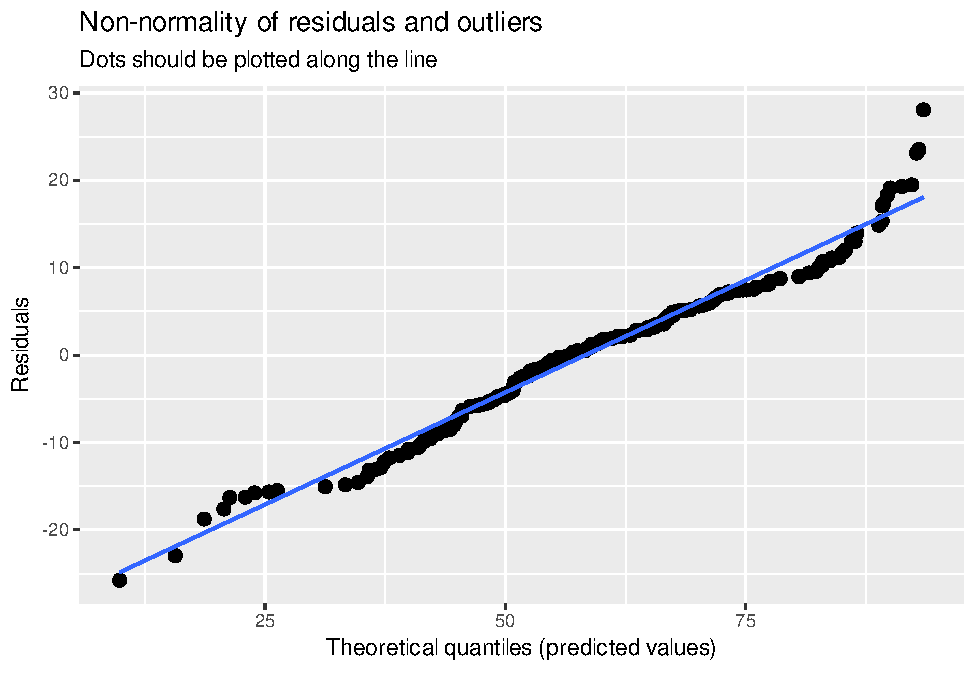
\includegraphics[width=0.25\linewidth]{OBIWAN_LIRA_files/figure-latex/unnamed-chunk-4-1} 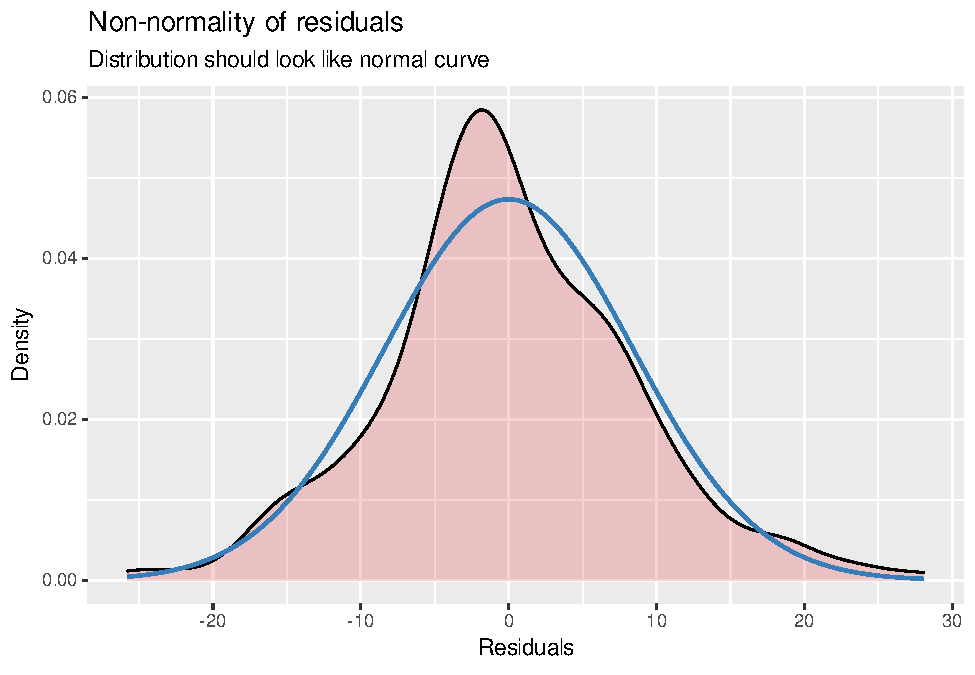
\includegraphics[width=0.25\linewidth]{OBIWAN_LIRA_files/figure-latex/unnamed-chunk-4-2} 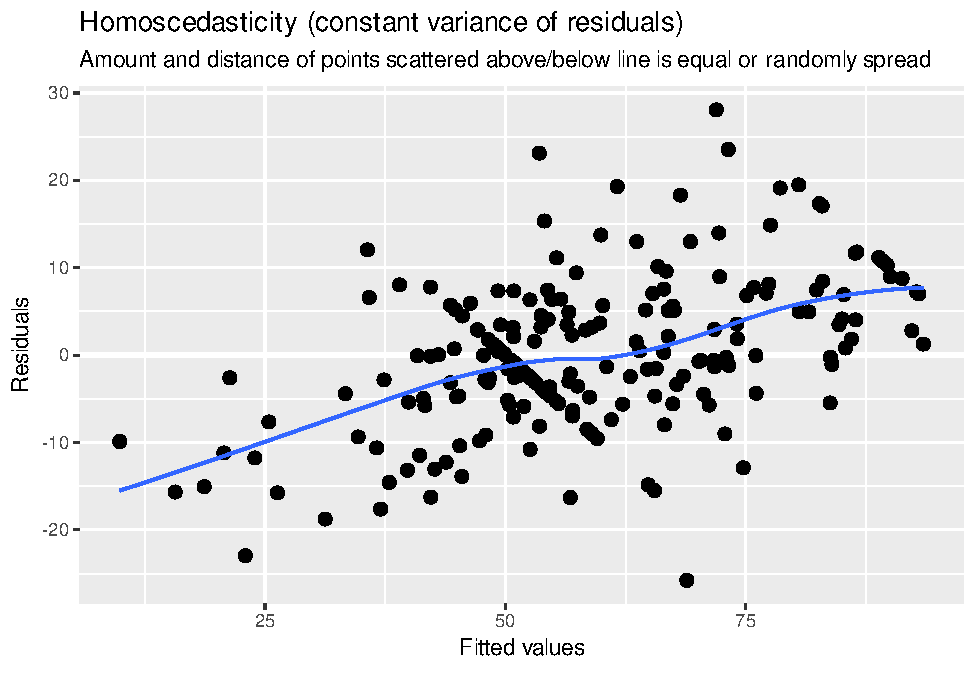
\includegraphics[width=0.25\linewidth]{OBIWAN_LIRA_files/figure-latex/unnamed-chunk-4-3} 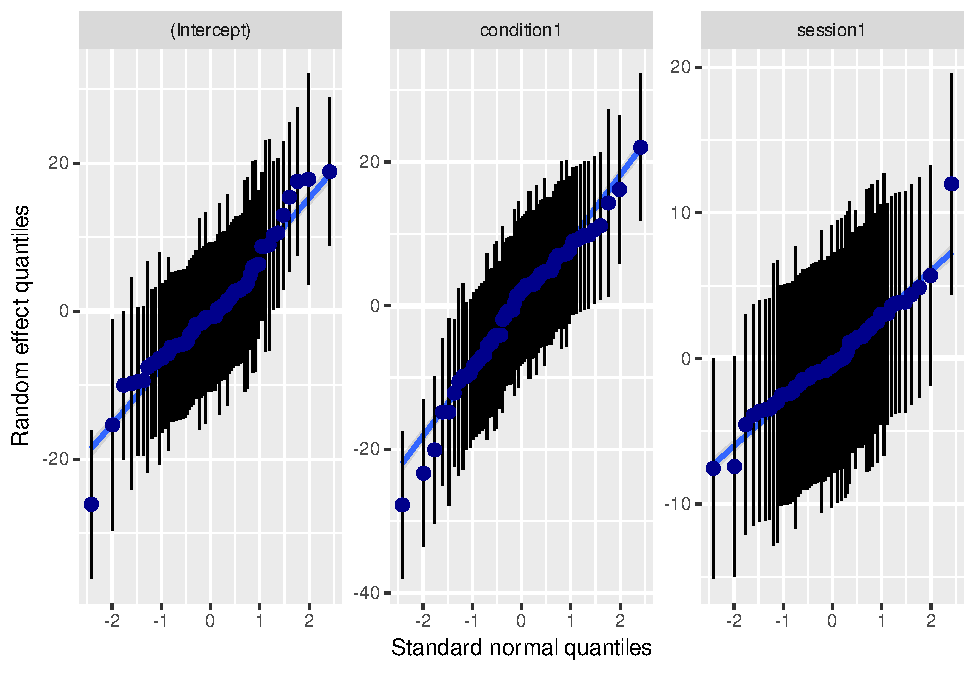
\includegraphics[width=0.25\linewidth]{OBIWAN_LIRA_files/figure-latex/unnamed-chunk-4-4} 

}

\caption{Model assumptions.}\label{fig:unnamed-chunk-4}
\end{figure}

\hfill\break
\hfill\break

\begin{figure}

{\centering 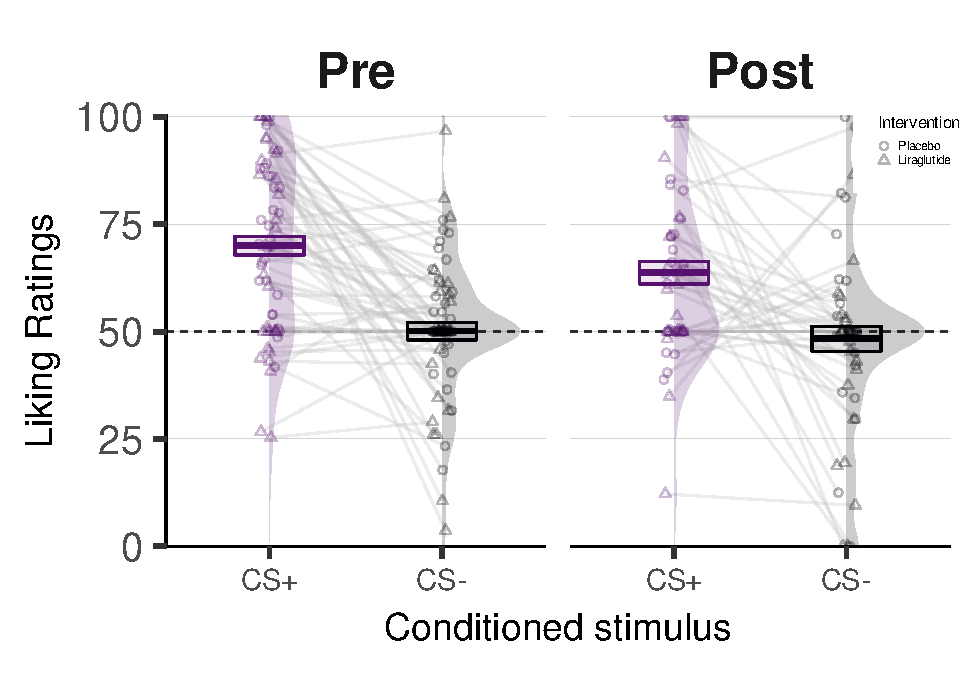
\includegraphics{OBIWAN_LIRA_files/figure-latex/PAV_LIK_plot-1} 

}

\caption{Pleasantness Ratings by pavlvovian cue.}\label{fig:PAV_LIK_plot}
\end{figure}

\hfill\break
\hfill\break

\hypertarget{instrumental-conditioning-task-analysis}{%
\subsection{Instrumental Conditioning Task
(Analysis)}\label{instrumental-conditioning-task-analysis}}

grips = number of times participant exceeded the force threshold to
acquire the reward (Milkshake) spline = first 5 trials (1st degree),
last 20 trials (2nd degree)

\begin{Shaded}
\begin{Highlighting}[]
\CommentTok{\#print(\textquotesingle{}BF10 for model piecewise regression model \textquotesingle{})}
\CommentTok{\#BF\_fit$BF[2]}
\NormalTok{BF\_fit}\SpecialCharTok{$}\NormalTok{Model }\OtherTok{=} \FunctionTok{c}\NormalTok{(}\StringTok{"Factorial early/late Learning Phasis"}\NormalTok{, }\StringTok{"Linear Time Fit"}\NormalTok{, }\StringTok{"Quadratic Time Fit"}\NormalTok{, }\StringTok{"Piecewise Regression with Splines"}\NormalTok{)}
\NormalTok{BF\_fit}\SpecialCharTok{$}\NormalTok{BF10 }\OtherTok{=} \FunctionTok{formatC}\NormalTok{(BF\_fit}\SpecialCharTok{$}\NormalTok{BF, }\AttributeTok{format =} \StringTok{"e"}\NormalTok{, }\AttributeTok{digits =} \DecValTok{2}\NormalTok{); BF\_fit}\SpecialCharTok{$}\NormalTok{BF10[}\DecValTok{1}\NormalTok{] }\OtherTok{=} \DecValTok{1}\NormalTok{; BF\_fit }\OtherTok{=}\NormalTok{ BF\_fit[}\SpecialCharTok{{-}}\FunctionTok{c}\NormalTok{(}\DecValTok{2}\NormalTok{)]}
\FunctionTok{kbl}\NormalTok{(}\FunctionTok{as\_tibble}\NormalTok{(BF\_fit), }\AttributeTok{caption =} \StringTok{"Bayesian Model Comparison"}\NormalTok{, }\AttributeTok{digits =} \DecValTok{1}\NormalTok{) }\SpecialCharTok{\%\textgreater{}\%}   \FunctionTok{kable\_styling}\NormalTok{(}\AttributeTok{latex\_options =} \StringTok{"HOLD\_position"}\NormalTok{, }\AttributeTok{position =} \StringTok{"center"}\NormalTok{, }\AttributeTok{full\_width =}\NormalTok{ F)  }\SpecialCharTok{\%\textgreater{}\%}  \FunctionTok{row\_spec}\NormalTok{(}\DecValTok{0}\NormalTok{,}\AttributeTok{bold=}\NormalTok{T,}\AttributeTok{align=}\StringTok{\textquotesingle{}c\textquotesingle{}}\NormalTok{)}
\end{Highlighting}
\end{Shaded}

\begin{table}[H]

\caption{\label{tab:INST_learning_MS}Bayesian Model Comparison}
\centering
\begin{tabular}[t]{l|l}
\hline
\multicolumn{1}{c}{\textbf{Model}} & \multicolumn{1}{c}{\textbf{BF10}}\\
\hline
Factorial early/late Learning Phasis & 1\\
\hline
Linear Time Fit & 1.41e+06\\
\hline
Quadratic Time Fit & 1.47e+04\\
\hline
Piecewise Regression with Splines & 1.05e+08\\
\hline
\end{tabular}
\end{table}

\hfill\break

\hfill\break

\begin{Shaded}
\begin{Highlighting}[]
\NormalTok{tables }\OtherTok{\textless{}{-}} \FunctionTok{list.clean}\NormalTok{(}\FunctionTok{readHTMLTable}\NormalTok{(}\StringTok{"tmp/temp3.html"}\NormalTok{), }\AttributeTok{fun =}\NormalTok{ is.null, }\AttributeTok{recursive =} \ConstantTok{FALSE}\NormalTok{)}
\NormalTok{tables2 }\OtherTok{=}\NormalTok{ tables[[}\DecValTok{1}\NormalTok{]] }\SpecialCharTok{\%\textgreater{}\%}\NormalTok{ janitor}\SpecialCharTok{::}\FunctionTok{row\_to\_names}\NormalTok{(}\AttributeTok{row\_number =} \DecValTok{1}\NormalTok{)}

\NormalTok{tables2 }\OtherTok{\textless{}{-}} \FunctionTok{as.matrix}\NormalTok{(tables2) }\SpecialCharTok{\%\textgreater{}\%} \FunctionTok{as\_tibble}\NormalTok{()}
\NormalTok{tables2[}\FunctionTok{is.na}\NormalTok{(tables2)] }\OtherTok{\textless{}{-}} \StringTok{""}
\NormalTok{tables3 }\OtherTok{=}\NormalTok{ tables2[}\DecValTok{1}\SpecialCharTok{:}\FunctionTok{length}\NormalTok{(table}\SpecialCharTok{$}\NormalTok{Effect),}\DecValTok{1}\SpecialCharTok{:}\DecValTok{4}\NormalTok{] }
\NormalTok{tables3[}\DecValTok{5}\NormalTok{] }\OtherTok{=} \FunctionTok{str\_split}\NormalTok{(}\FunctionTok{gsub}\NormalTok{(}\StringTok{"[\^{}0{-}9.,{-}]"}\NormalTok{, }\StringTok{""}\NormalTok{, table[}\DecValTok{3}\NormalTok{]), }\StringTok{","}\NormalTok{)[[}\DecValTok{1}\NormalTok{]]; tables3[}\DecValTok{6}\NormalTok{] }\OtherTok{=} \FunctionTok{as.numeric}\NormalTok{(}\FunctionTok{str\_split}\NormalTok{(}\FunctionTok{gsub}\NormalTok{(}\StringTok{"[\^{}0{-}9.,{-}]"}\NormalTok{, }\StringTok{""}\NormalTok{, table[}\DecValTok{4}\NormalTok{]), }\StringTok{","}\NormalTok{)[[}\DecValTok{1}\NormalTok{]]); }
\NormalTok{tables3}\SpecialCharTok{$}\NormalTok{...}\DecValTok{6} \OtherTok{=} \FunctionTok{ifelse}\NormalTok{(tables3}\SpecialCharTok{$}\NormalTok{...}\DecValTok{6} \SpecialCharTok{\textless{}} \FloatTok{0.05}\NormalTok{,}\FunctionTok{paste}\NormalTok{(}\StringTok{"\textless{}span style=}\SpecialCharTok{\textbackslash{}"}\StringTok{ font{-}weight: bold; }\SpecialCharTok{\textbackslash{}"}\StringTok{ \textgreater{}"}\NormalTok{ ,}\FunctionTok{sprintf}\NormalTok{(}\StringTok{"\%.3f"}\NormalTok{,tables3}\SpecialCharTok{$}\NormalTok{...}\DecValTok{6}\NormalTok{), }\StringTok{"\textless{}/span\textgreater{}"}\NormalTok{),  }\FunctionTok{paste}\NormalTok{(}\StringTok{"\textless{}span\textgreater{}"}\NormalTok{ ,}\FunctionTok{sprintf}\NormalTok{(}\StringTok{"\%.3f"}\NormalTok{,tables3}\SpecialCharTok{$}\NormalTok{...}\DecValTok{6}\NormalTok{), }\StringTok{"\textless{}/span\textgreater{}"}\NormalTok{))}

\FunctionTok{colnames}\NormalTok{(tables3)[}\DecValTok{5}\NormalTok{] }\OtherTok{=} \StringTok{"\textbackslash{}u03C7\textbackslash{}u00B2"}\NormalTok{; }\FunctionTok{colnames}\NormalTok{(tables3)[}\DecValTok{6}\NormalTok{] }\OtherTok{=} \StringTok{"p"}
\CommentTok{\# tables3$p[3]= "\textless{}span style=\textbackslash{}" font{-}weight: bold;    \textbackslash{}" \textgreater{}\textbackslash{}u003C 0.300\textless{}/span\textgreater{}"}
\NormalTok{tables3 }\SpecialCharTok{\%\textgreater{}\%} \FunctionTok{kbl}\NormalTok{(}\AttributeTok{caption =}\StringTok{"Grips"}\NormalTok{,}\AttributeTok{escape =}\NormalTok{ F ) }\SpecialCharTok{\%\textgreater{}\%}
  \FunctionTok{kable\_styling}\NormalTok{(}\AttributeTok{latex\_options =} \StringTok{"HOLD\_position"}\NormalTok{, }\AttributeTok{position =} \StringTok{"center"}\NormalTok{, }\AttributeTok{full\_width =}\NormalTok{ F) }\SpecialCharTok{\%\textgreater{}\%}  \FunctionTok{row\_spec}\NormalTok{(}\DecValTok{0}\NormalTok{,}\AttributeTok{bold=}\NormalTok{T,}\AttributeTok{align=}\StringTok{\textquotesingle{}c\textquotesingle{}}\NormalTok{)}
\end{Highlighting}
\end{Shaded}

\begin{table}[H]

\caption{\label{tab:INST_mod}Grips}
\centering
\begin{tabular}[t]{l|l|l|l|l|l}
\hline
\multicolumn{1}{c}{\textbf{Predictors}} & \multicolumn{1}{c}{\textbf{Estimates}} & \multicolumn{1}{c}{\textbf{std. Error}} & \multicolumn{1}{c}{\textbf{CI}} & \multicolumn{1}{c}{\textbf{χ²}} & \multicolumn{1}{c}{\textbf{p}}\\
\hline
intervention [1] & 0.32 & 0.76 & -1.17 – 1.80 & 0.17 & <span> 0.678 </span>\\
\hline
session [1] & -0.38 & 0.38 & -1.13 – 0.37 & 0.98 & <span> 0.321 </span>\\
\hline
age & -0.80 & 0.76 & -2.29 – 0.69 & 1.08 & <span> 0.300 </span>\\
\hline
gender [1] & 0.64 & 0.81 & -0.95 – 2.22 & 0.62 & <span> 0.432 </span>\\
\hline
BMI_V1 & -0.82 & 0.83 & -2.44 – 0.80 & 0.96 & <span> 0.326 </span>\\
\hline
thirsty & 1.39 & 0.65 & 0.12 – 2.65 & 4.40 & <span style=" font-weight: bold; " > 0.036 </span>\\
\hline
hungry & -0.74 & 0.70 & -2.10 – 0.62 & 1.06 & <span> 0.304 </span>\\
\hline
intervention [1] *session [1] & -0.41 & 0.39 & -1.17 – 0.35 & 1.09 & <span> 0.297 </span>\\
\hline
session [1] * thirsty & -0.72 & 0.44 & -1.58 – 0.14 & 2.65 & <span> 0.103 </span>\\
\hline
\end{tabular}
\end{table}

\begin{Shaded}
\begin{Highlighting}[]
\NormalTok{tmp }\OtherTok{=}\NormalTok{ tables2[(}\FunctionTok{length}\NormalTok{(table}\SpecialCharTok{$}\NormalTok{Effect)}\SpecialCharTok{+}\DecValTok{1}\NormalTok{)}\SpecialCharTok{:}\NormalTok{(}\FunctionTok{length}\NormalTok{(table}\SpecialCharTok{$}\NormalTok{Effect)}\SpecialCharTok{+}\DecValTok{5}\NormalTok{),}\DecValTok{1}\SpecialCharTok{:}\DecValTok{2}\NormalTok{]}
\FunctionTok{names}\NormalTok{(tmp) }\OtherTok{\textless{}{-}} \ConstantTok{NULL}
\NormalTok{tmp1 }\OtherTok{\textless{}{-}} \FunctionTok{data.frame}\NormalTok{(}\FunctionTok{t}\NormalTok{(tmp[}\SpecialCharTok{{-}}\DecValTok{1}\NormalTok{]))}
\FunctionTok{colnames}\NormalTok{(tmp1) }\OtherTok{\textless{}{-}}\NormalTok{ tmp[[}\DecValTok{1}\NormalTok{]]}
\NormalTok{tmp1 }\SpecialCharTok{\%\textgreater{}\%} \FunctionTok{kbl}\NormalTok{(}\AttributeTok{digits =} \DecValTok{2}\NormalTok{) }\SpecialCharTok{\%\textgreater{}\%}
  \FunctionTok{kable\_styling}\NormalTok{(}\AttributeTok{latex\_options =} \StringTok{"HOLD\_position"}\NormalTok{, }\AttributeTok{position =} \StringTok{"center"}\NormalTok{, }\AttributeTok{full\_width =}\NormalTok{ F) }
\end{Highlighting}
\end{Shaded}

\begin{table}[H]
\centering
\begin{tabular}[t]{l|l|l|l|l}
\hline
ICC & N id & N trial & Observations & Marginal R2 / Conditional R2\\
\hline
0.78 & 63 & 24 & 2640 & 0.067 / 0.793\\
\hline
\end{tabular}
\end{table}

\hfill\break

\begin{figure}

{\centering 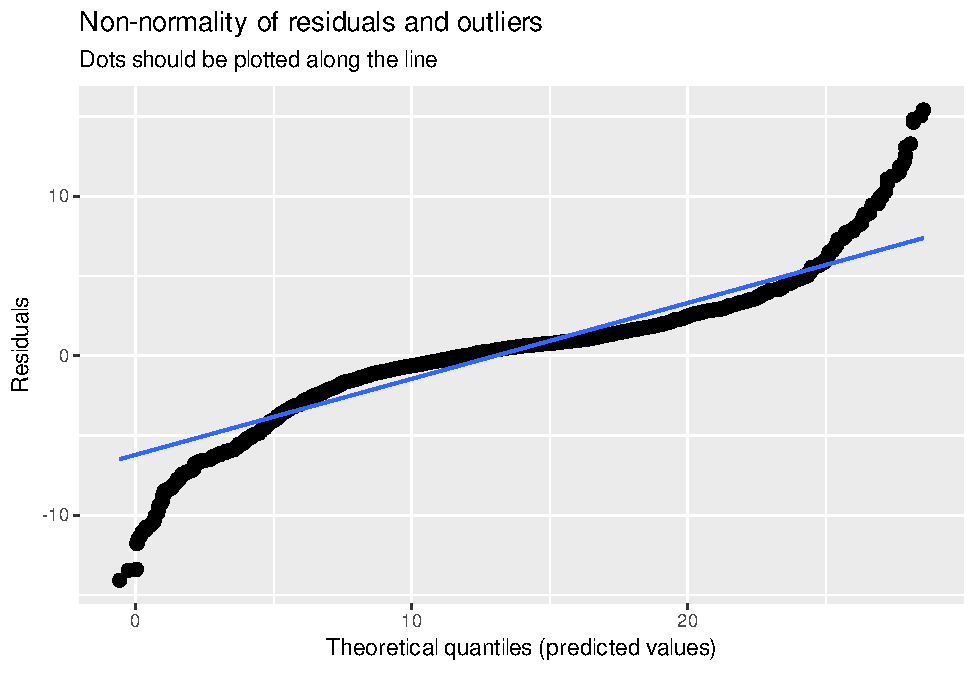
\includegraphics[width=0.25\linewidth]{OBIWAN_LIRA_files/figure-latex/unnamed-chunk-5-1} 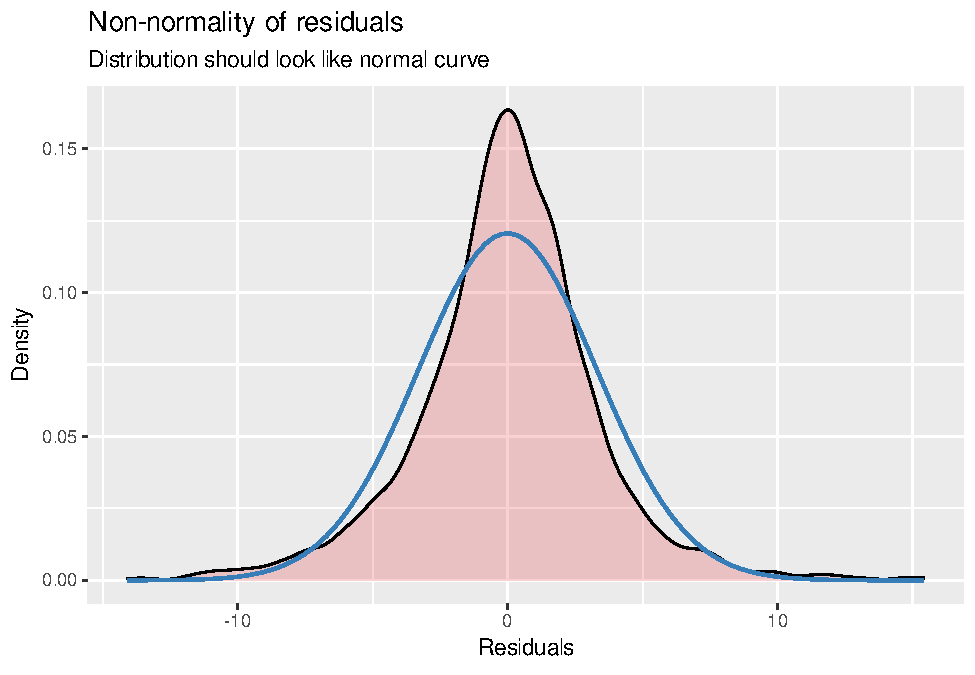
\includegraphics[width=0.25\linewidth]{OBIWAN_LIRA_files/figure-latex/unnamed-chunk-5-2} 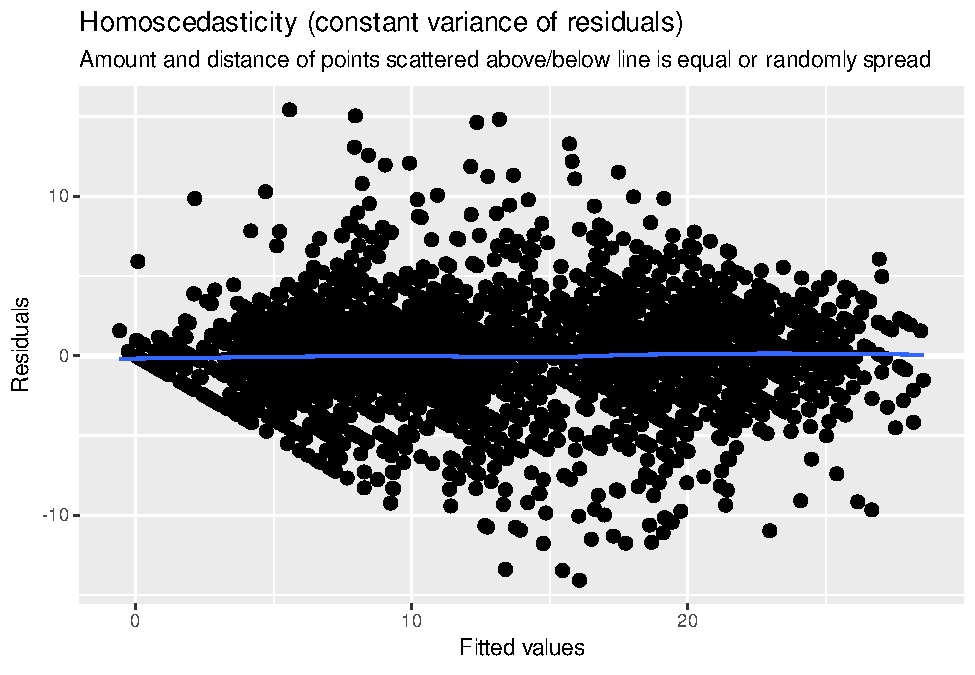
\includegraphics[width=0.25\linewidth]{OBIWAN_LIRA_files/figure-latex/unnamed-chunk-5-3} 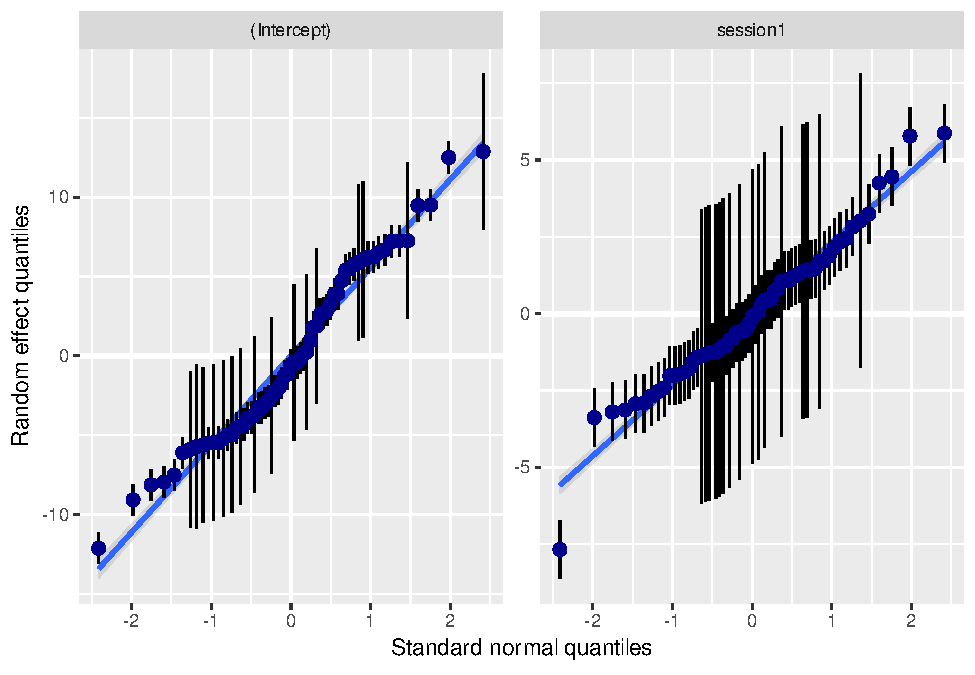
\includegraphics[width=0.25\linewidth]{OBIWAN_LIRA_files/figure-latex/unnamed-chunk-5-4} 

}

\caption{Model assumptions.}\label{fig:unnamed-chunk-5}
\end{figure}

\hfill\break
\hfill\break

\begin{figure}

{\centering 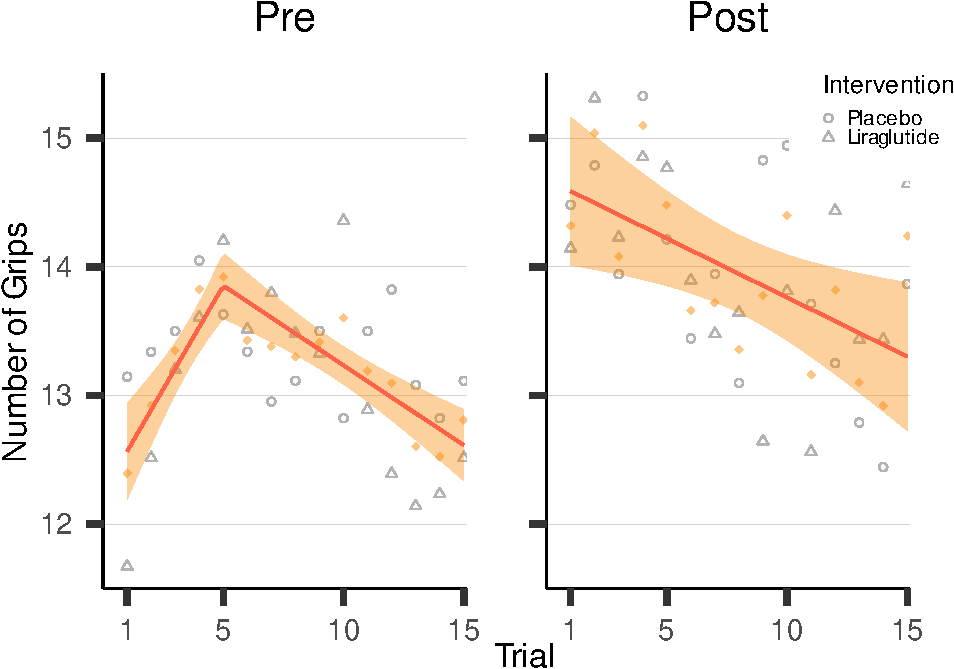
\includegraphics{OBIWAN_LIRA_files/figure-latex/INST_plot-1} 

}

\caption{Number of Grips over time by session.}\label{fig:INST_plot}
\end{figure}

\hfill\break
\hfill\break

\hypertarget{pit-pavlovian-instrumental-transfer-task}{%
\subsection{PIT (Pavlovian-Instrumental Transfer)
Task}\label{pit-pavlovian-instrumental-transfer-task}}

Mobilized effort = Area Under the Curve (AUC) of the force exerted
exceeding the delivery threshold during Pavlvovian cue presentation
condition = CS+ or CS-

\hfill\break

\begin{Shaded}
\begin{Highlighting}[]
\NormalTok{tables }\OtherTok{\textless{}{-}} \FunctionTok{list.clean}\NormalTok{(}\FunctionTok{readHTMLTable}\NormalTok{(}\StringTok{"tmp/temp4.html"}\NormalTok{), }\AttributeTok{fun =}\NormalTok{ is.null, }\AttributeTok{recursive =} \ConstantTok{FALSE}\NormalTok{)}
\NormalTok{tables2 }\OtherTok{=}\NormalTok{ tables[[}\DecValTok{1}\NormalTok{]] }\SpecialCharTok{\%\textgreater{}\%}\NormalTok{ janitor}\SpecialCharTok{::}\FunctionTok{row\_to\_names}\NormalTok{(}\AttributeTok{row\_number =} \DecValTok{1}\NormalTok{)}

\NormalTok{tables2 }\OtherTok{\textless{}{-}} \FunctionTok{as.matrix}\NormalTok{(tables2) }\SpecialCharTok{\%\textgreater{}\%} \FunctionTok{as\_tibble}\NormalTok{()}
\NormalTok{tables2[}\FunctionTok{is.na}\NormalTok{(tables2)] }\OtherTok{\textless{}{-}} \StringTok{""}
\NormalTok{tables3 }\OtherTok{=}\NormalTok{ tables2[}\DecValTok{1}\SpecialCharTok{:}\FunctionTok{length}\NormalTok{(table}\SpecialCharTok{$}\NormalTok{Effect),}\DecValTok{1}\SpecialCharTok{:}\DecValTok{4}\NormalTok{] }
\NormalTok{tables3[}\DecValTok{5}\NormalTok{] }\OtherTok{=} \FunctionTok{str\_split}\NormalTok{(}\FunctionTok{gsub}\NormalTok{(}\StringTok{"[\^{}0{-}9.,{-}]"}\NormalTok{, }\StringTok{""}\NormalTok{, table[}\DecValTok{3}\NormalTok{]), }\StringTok{","}\NormalTok{)[[}\DecValTok{1}\NormalTok{]]; tables3[}\DecValTok{6}\NormalTok{] }\OtherTok{=} \FunctionTok{as.numeric}\NormalTok{(}\FunctionTok{str\_split}\NormalTok{(}\FunctionTok{gsub}\NormalTok{(}\StringTok{"[\^{}0{-}9.,{-}]"}\NormalTok{, }\StringTok{""}\NormalTok{, table[}\DecValTok{4}\NormalTok{]), }\StringTok{","}\NormalTok{)[[}\DecValTok{1}\NormalTok{]]); }
\NormalTok{tables3}\SpecialCharTok{$}\NormalTok{...}\DecValTok{6} \OtherTok{=} \FunctionTok{ifelse}\NormalTok{(tables3}\SpecialCharTok{$}\NormalTok{...}\DecValTok{6} \SpecialCharTok{\textless{}} \FloatTok{0.05}\NormalTok{,}\FunctionTok{paste}\NormalTok{(}\StringTok{"\textless{}span style=}\SpecialCharTok{\textbackslash{}"}\StringTok{ font{-}weight: bold; }\SpecialCharTok{\textbackslash{}"}\StringTok{ \textgreater{}"}\NormalTok{ ,}\FunctionTok{sprintf}\NormalTok{(}\StringTok{"\%.3f"}\NormalTok{,tables3}\SpecialCharTok{$}\NormalTok{...}\DecValTok{6}\NormalTok{), }\StringTok{"\textless{}/span\textgreater{}"}\NormalTok{),  }\FunctionTok{paste}\NormalTok{(}\StringTok{"\textless{}span\textgreater{}"}\NormalTok{ ,}\FunctionTok{sprintf}\NormalTok{(}\StringTok{"\%.3f"}\NormalTok{,tables3}\SpecialCharTok{$}\NormalTok{...}\DecValTok{6}\NormalTok{), }\StringTok{"\textless{}/span\textgreater{}"}\NormalTok{))}
\FunctionTok{colnames}\NormalTok{(tables3)[}\DecValTok{5}\NormalTok{] }\OtherTok{=} \StringTok{"\textbackslash{}u03C7\textbackslash{}u00B2"}\NormalTok{; }\FunctionTok{colnames}\NormalTok{(tables3)[}\DecValTok{6}\NormalTok{] }\OtherTok{=} \StringTok{"p"}
\CommentTok{\#tables3$p[1]= "\textless{}span style=\textbackslash{}" font{-}weight: bold;    \textbackslash{}" \textgreater{}\textbackslash{}u003C 0.001\textless{}/span\textgreater{}"}
\NormalTok{tables3  }\SpecialCharTok{\%\textgreater{}\%} \FunctionTok{kbl}\NormalTok{(}\AttributeTok{caption =}\StringTok{"Mobilized effort (a.u.)"}\NormalTok{,}\AttributeTok{escape =}\NormalTok{ F ) }\SpecialCharTok{\%\textgreater{}\%}
  \FunctionTok{kable\_styling}\NormalTok{(}\AttributeTok{latex\_options =} \StringTok{"HOLD\_position"}\NormalTok{, }\AttributeTok{position =} \StringTok{"center"}\NormalTok{, }\AttributeTok{full\_width =}\NormalTok{ F) }\SpecialCharTok{\%\textgreater{}\%}  \FunctionTok{row\_spec}\NormalTok{(}\DecValTok{0}\NormalTok{,}\AttributeTok{bold=}\NormalTok{T,}\AttributeTok{align=}\StringTok{\textquotesingle{}c\textquotesingle{}}\NormalTok{)}
\end{Highlighting}
\end{Shaded}

\begin{table}[H]

\caption{\label{tab:PIT_mod}Mobilized effort (a.u.)}
\centering
\begin{tabular}[t]{l|l|l|l|l|l}
\hline
\multicolumn{1}{c}{\textbf{Predictors}} & \multicolumn{1}{c}{\textbf{Estimates}} & \multicolumn{1}{c}{\textbf{std. Error}} & \multicolumn{1}{c}{\textbf{CI}} & \multicolumn{1}{c}{\textbf{χ²}} & \multicolumn{1}{c}{\textbf{p}}\\
\hline
condition [1] & -7.81 & 3.19 & -14.07 – -1.55 & 5.66 & <span style=" font-weight: bold; " > 0.017 </span>\\
\hline
intervention [1] & -5.79 & 10.01 & -25.41 – 13.83 & 0.33 & <span> 0.564 </span>\\
\hline
session [1] & -0.36 & 7.00 & -14.07 – 13.36 & 0.00 & <span> 0.959 </span>\\
\hline
age & 27.40 & 9.89 & 8.01 – 46.79 & 7.08 & <span style=" font-weight: bold; " > 0.008 </span>\\
\hline
gender [1] & 3.62 & 10.34 & -16.65 – 23.90 & 0.10 & <span> 0.750 </span>\\
\hline
BMI_V1 & -14.97 & 10.18 & -34.92 – 4.97 & 2.01 & <span> 0.157 </span>\\
\hline
thirsty & 3.25 & 9.48 & -15.33 – 21.82 & 0.11 & <span> 0.742 </span>\\
\hline
hungry & 5.45 & 9.86 & -13.89 – 24.78 & 0.27 & <span> 0.601 </span>\\
\hline
condition [1] *intervention [1] & 0.18 & 3.19 & -6.08 – 6.44 & 0.00 & <span> 0.956 </span>\\
\hline
condition [1] * session[1] & 1.87 & 2.46 & -2.95 – 6.70 & 0.57 & <span> 0.450 </span>\\
\hline
intervention [1] *session [1] & 3.78 & 6.99 & -9.92 – 17.49 & 0.29 & <span> 0.589 </span>\\
\hline
(condition [1] *intervention [1]) *session [1] & -2.24 & 2.46 & -7.07 – 2.59 & 0.82 & <span> 0.366 </span>\\
\hline
\end{tabular}
\end{table}

\begin{Shaded}
\begin{Highlighting}[]
\NormalTok{tmp }\OtherTok{=}\NormalTok{ tables2[(}\FunctionTok{length}\NormalTok{(table}\SpecialCharTok{$}\NormalTok{Effect)}\SpecialCharTok{+}\DecValTok{1}\NormalTok{)}\SpecialCharTok{:}\NormalTok{(}\FunctionTok{length}\NormalTok{(table}\SpecialCharTok{$}\NormalTok{Effect)}\SpecialCharTok{+}\DecValTok{5}\NormalTok{),}\DecValTok{1}\SpecialCharTok{:}\DecValTok{2}\NormalTok{]}
\FunctionTok{names}\NormalTok{(tmp) }\OtherTok{\textless{}{-}} \ConstantTok{NULL}
\NormalTok{tmp1 }\OtherTok{\textless{}{-}} \FunctionTok{data.frame}\NormalTok{(}\FunctionTok{t}\NormalTok{(tmp[}\SpecialCharTok{{-}}\DecValTok{1}\NormalTok{]))}
\FunctionTok{colnames}\NormalTok{(tmp1) }\OtherTok{\textless{}{-}}\NormalTok{ tmp[[}\DecValTok{1}\NormalTok{]]}
\NormalTok{tmp1 }\SpecialCharTok{\%\textgreater{}\%} \FunctionTok{kbl}\NormalTok{(}\AttributeTok{digits =} \DecValTok{2}\NormalTok{) }\SpecialCharTok{\%\textgreater{}\%}
  \FunctionTok{kable\_styling}\NormalTok{(}\AttributeTok{latex\_options =} \StringTok{"HOLD\_position"}\NormalTok{, }\AttributeTok{position =} \StringTok{"center"}\NormalTok{, }\AttributeTok{full\_width =}\NormalTok{ F) }
\end{Highlighting}
\end{Shaded}

\begin{table}[H]
\centering
\begin{tabular}[t]{l|l|l|l|l}
\hline
ICC & N id & N trialxcondition & Observations & Marginal R2 / Conditional R2\\
\hline
0.75 & 64 & 15 & 3300 & 0.073 / 0.771\\
\hline
\end{tabular}
\end{table}

\hfill\break

\begin{figure}

{\centering 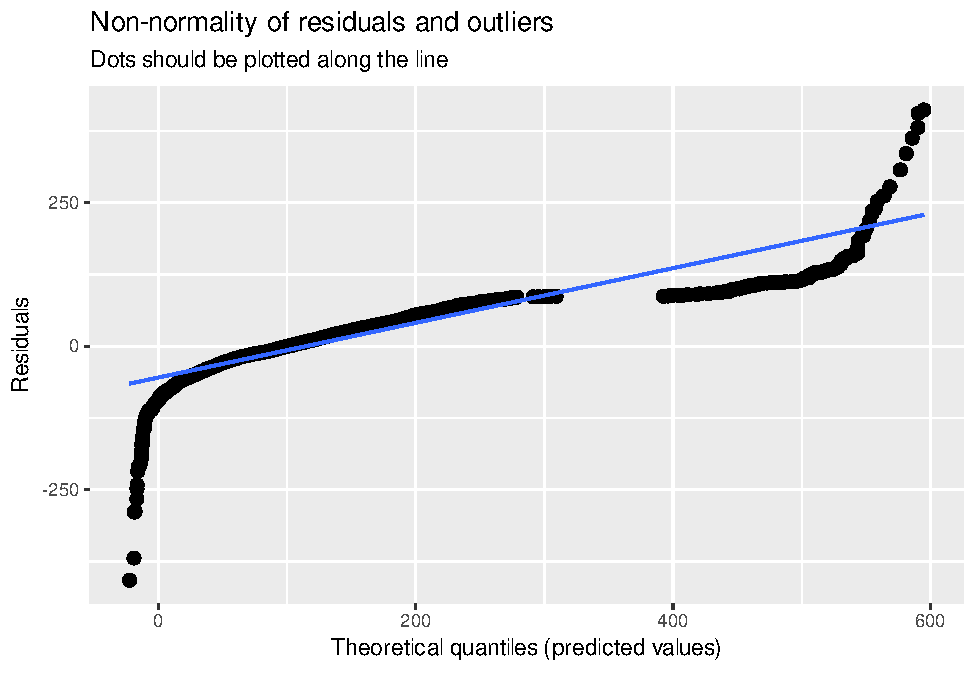
\includegraphics[width=0.25\linewidth]{OBIWAN_LIRA_files/figure-latex/unnamed-chunk-6-1} 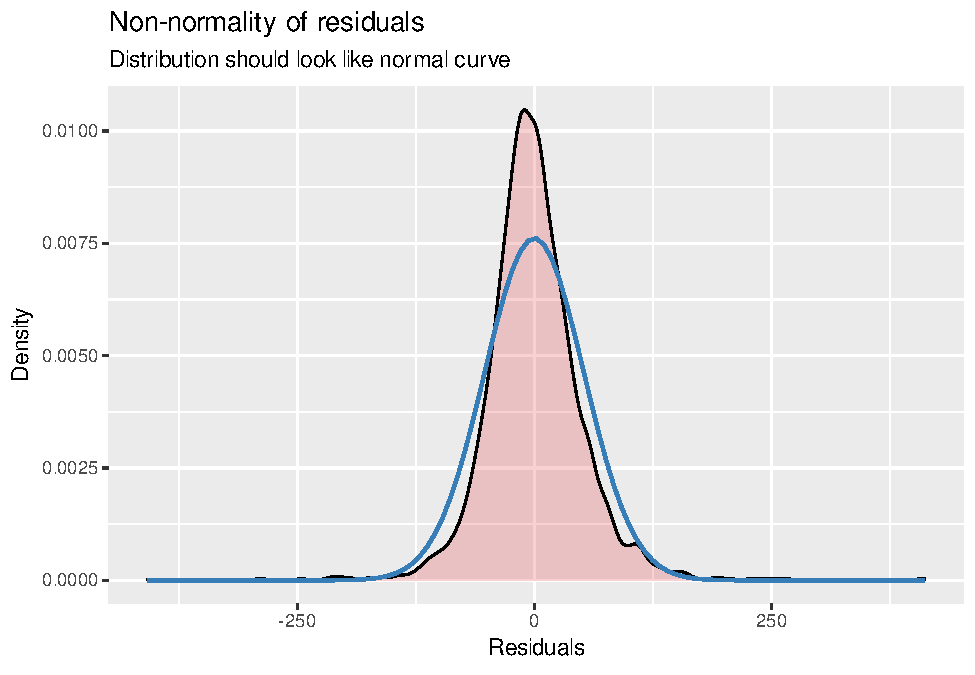
\includegraphics[width=0.25\linewidth]{OBIWAN_LIRA_files/figure-latex/unnamed-chunk-6-2} 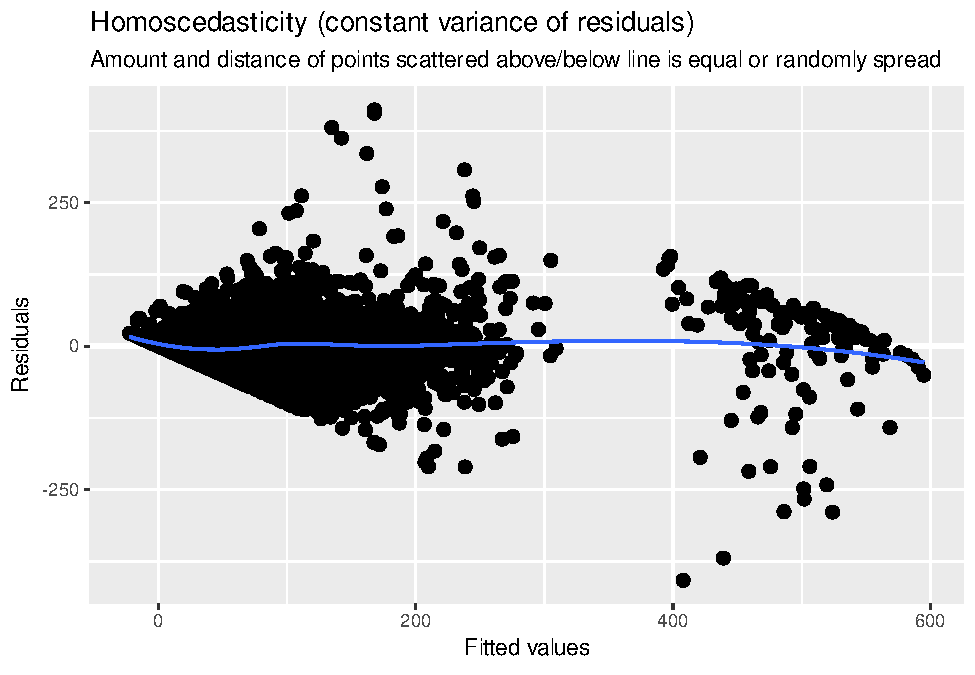
\includegraphics[width=0.25\linewidth]{OBIWAN_LIRA_files/figure-latex/unnamed-chunk-6-3} 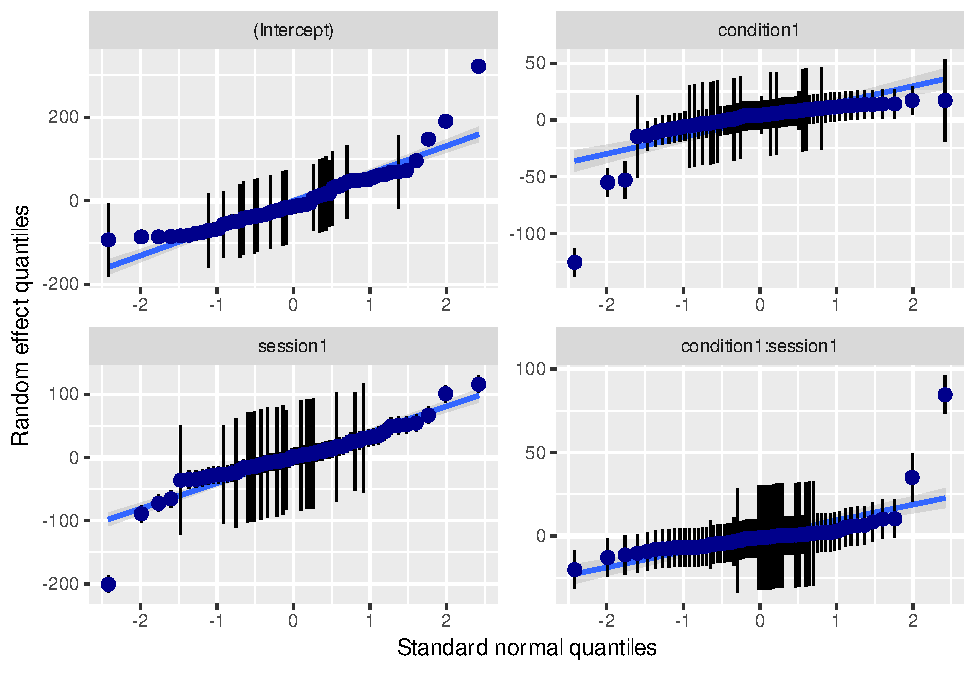
\includegraphics[width=0.25\linewidth]{OBIWAN_LIRA_files/figure-latex/unnamed-chunk-6-4} 

}

\caption{Model assumptions.}\label{fig:unnamed-chunk-6}
\end{figure}

\hfill\break
\hfill\break

\begin{figure}

{\centering 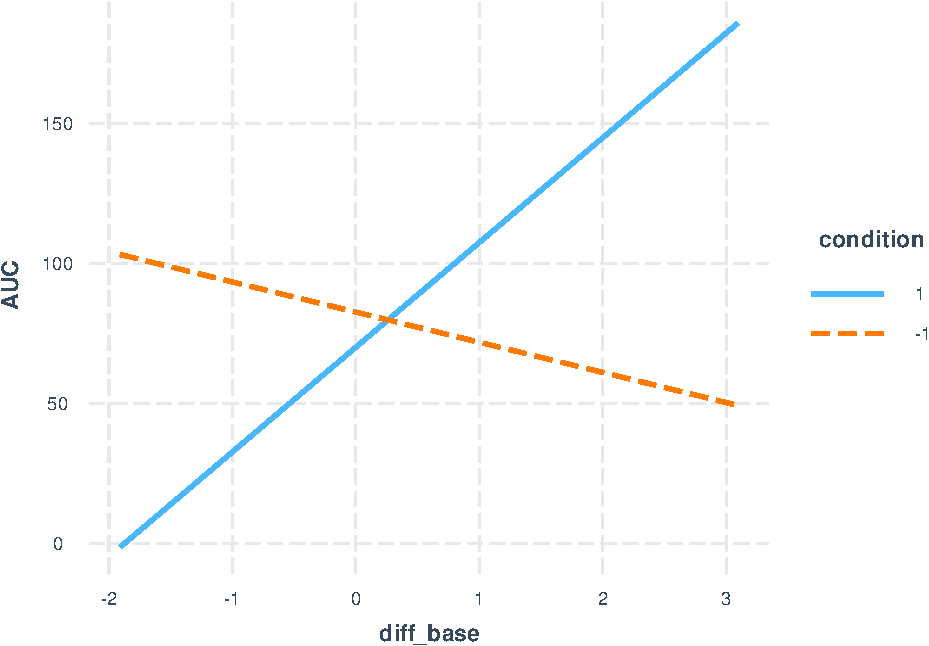
\includegraphics{OBIWAN_LIRA_files/figure-latex/PIT_plot-1} 

}

\caption{Mobilized effort by pavlovian cue.}\label{fig:PIT_plot}
\end{figure}

\hfill\break
\hfill\break

\hypertarget{hedonic-reactivity-test}{%
\subsection{Hedonic Reactivity Test}\label{hedonic-reactivity-test}}

Perceived liking = how pleasant is the liquid solution rated (0-100,
with repetitions) \& condition = Milshake or Tasteless \& intensity =
difference on how intense the liquid solution were rated

\hfill\break

\begin{Shaded}
\begin{Highlighting}[]
\NormalTok{tables }\OtherTok{\textless{}{-}} \FunctionTok{list.clean}\NormalTok{(}\FunctionTok{readHTMLTable}\NormalTok{(}\StringTok{"tmp/temp5.html"}\NormalTok{), }\AttributeTok{fun =}\NormalTok{ is.null, }\AttributeTok{recursive =} \ConstantTok{FALSE}\NormalTok{)}
\NormalTok{tables2 }\OtherTok{=}\NormalTok{ tables[[}\DecValTok{1}\NormalTok{]] }\SpecialCharTok{\%\textgreater{}\%}\NormalTok{ janitor}\SpecialCharTok{::}\FunctionTok{row\_to\_names}\NormalTok{(}\AttributeTok{row\_number =} \DecValTok{1}\NormalTok{)}

\NormalTok{tables2 }\OtherTok{\textless{}{-}} \FunctionTok{as.matrix}\NormalTok{(tables2) }\SpecialCharTok{\%\textgreater{}\%} \FunctionTok{as\_tibble}\NormalTok{()}
\NormalTok{tables2[}\FunctionTok{is.na}\NormalTok{(tables2)] }\OtherTok{\textless{}{-}} \StringTok{""}
\NormalTok{tables3 }\OtherTok{=}\NormalTok{ tables2[}\DecValTok{1}\SpecialCharTok{:}\FunctionTok{length}\NormalTok{(table}\SpecialCharTok{$}\NormalTok{Effect),}\DecValTok{1}\SpecialCharTok{:}\DecValTok{4}\NormalTok{] }
\NormalTok{tables3[}\DecValTok{5}\NormalTok{] }\OtherTok{=} \FunctionTok{str\_split}\NormalTok{(}\FunctionTok{gsub}\NormalTok{(}\StringTok{"[\^{}0{-}9.,{-}]"}\NormalTok{, }\StringTok{""}\NormalTok{, table[}\DecValTok{3}\NormalTok{]), }\StringTok{","}\NormalTok{)[[}\DecValTok{1}\NormalTok{]]; tables3[}\DecValTok{6}\NormalTok{] }\OtherTok{=} \FunctionTok{as.numeric}\NormalTok{(}\FunctionTok{str\_split}\NormalTok{(}\FunctionTok{gsub}\NormalTok{(}\StringTok{"[\^{}0{-}9.,{-}]"}\NormalTok{, }\StringTok{""}\NormalTok{, table[}\DecValTok{4}\NormalTok{]), }\StringTok{","}\NormalTok{)[[}\DecValTok{1}\NormalTok{]]); }
\NormalTok{tables3}\SpecialCharTok{$}\NormalTok{...}\DecValTok{6} \OtherTok{=} \FunctionTok{ifelse}\NormalTok{(tables3}\SpecialCharTok{$}\NormalTok{...}\DecValTok{6} \SpecialCharTok{\textless{}} \FloatTok{0.05}\NormalTok{,}\FunctionTok{paste}\NormalTok{(}\StringTok{"\textless{}span style=}\SpecialCharTok{\textbackslash{}"}\StringTok{ font{-}weight: bold; }\SpecialCharTok{\textbackslash{}"}\StringTok{ \textgreater{}"}\NormalTok{ ,}\FunctionTok{sprintf}\NormalTok{(}\StringTok{"\%.3f"}\NormalTok{,tables3}\SpecialCharTok{$}\NormalTok{...}\DecValTok{6}\NormalTok{), }\StringTok{"\textless{}/span\textgreater{}"}\NormalTok{),  }\FunctionTok{paste}\NormalTok{(}\StringTok{"\textless{}span\textgreater{}"}\NormalTok{ ,}\FunctionTok{sprintf}\NormalTok{(}\StringTok{"\%.3f"}\NormalTok{,tables3}\SpecialCharTok{$}\NormalTok{...}\DecValTok{6}\NormalTok{), }\StringTok{"\textless{}/span\textgreater{}"}\NormalTok{))}
\FunctionTok{colnames}\NormalTok{(tables3)[}\DecValTok{5}\NormalTok{] }\OtherTok{=} \StringTok{"\textbackslash{}u03C7\textbackslash{}u00B2"}\NormalTok{; }\FunctionTok{colnames}\NormalTok{(tables3)[}\DecValTok{6}\NormalTok{] }\OtherTok{=} \StringTok{"p"}
\NormalTok{tables3}\SpecialCharTok{$}\NormalTok{p[}\DecValTok{1}\NormalTok{]}\OtherTok{=} \StringTok{"\textless{}span style=}\SpecialCharTok{\textbackslash{}"}\StringTok{ font{-}weight: bold;    }\SpecialCharTok{\textbackslash{}"}\StringTok{ \textgreater{}\textbackslash{}u003C 0.001\textless{}/span\textgreater{}"}
\NormalTok{tables3  }\SpecialCharTok{\%\textgreater{}\%} \FunctionTok{kbl}\NormalTok{(}\AttributeTok{caption =}\StringTok{"Perceived liking"}\NormalTok{,}\AttributeTok{escape =}\NormalTok{ F ) }\SpecialCharTok{\%\textgreater{}\%}
  \FunctionTok{kable\_styling}\NormalTok{(}\AttributeTok{latex\_options =} \StringTok{"HOLD\_position"}\NormalTok{, }\AttributeTok{position =} \StringTok{"center"}\NormalTok{, }\AttributeTok{full\_width =}\NormalTok{ F) }\SpecialCharTok{\%\textgreater{}\%}  \FunctionTok{row\_spec}\NormalTok{(}\DecValTok{0}\NormalTok{,}\AttributeTok{bold=}\NormalTok{T,}\AttributeTok{align=}\StringTok{\textquotesingle{}c\textquotesingle{}}\NormalTok{)}
\end{Highlighting}
\end{Shaded}

\begin{table}[H]

\caption{\label{tab:HED_mod}Perceived liking}
\centering
\begin{tabular}[t]{l|l|l|l|l|l}
\hline
\multicolumn{1}{c}{\textbf{Predictors}} & \multicolumn{1}{c}{\textbf{Estimates}} & \multicolumn{1}{c}{\textbf{std. Error}} & \multicolumn{1}{c}{\textbf{CI}} & \multicolumn{1}{c}{\textbf{χ²}} & \multicolumn{1}{c}{\textbf{p}}\\
\hline
condition [1] & -6.57 & 1.37 & -9.25 – -3.89 & 80.15 & <span style=" font-weight: bold;    " >< 0.001</span>\\
\hline
intervention [1] & -0.18 & 1.37 & -2.87 – 2.50 & 0.00 & <span> 0.999 </span>\\
\hline
session [1] & 2.70 & 0.89 & 0.95 – 4.45 & 0.00 & <span> 0.999 </span>\\
\hline
age & 0.69 & 1.20 & -1.67 – 3.05 & 0.00 & <span> 0.966 </span>\\
\hline
gender [1] & -2.34 & 1.26 & -4.81 – 0.13 & 1.91 & <span> 0.167 </span>\\
\hline
BMI_V1 & -0.77 & 1.24 & -3.20 – 1.65 & 1.60 & <span> 0.206 </span>\\
\hline
thirsty & -0.73 & 1.16 & -3.00 – 1.54 & 11.01 & <span style=" font-weight: bold; " > 0.001 </span>\\
\hline
hungry & 2.08 & 1.18 & -0.24 – 4.39 & 0.85 & <span> 0.357 </span>\\
\hline
int & 0.37 & 1.13 & -1.84 – 2.58 & 0.00 & <span> 0.999 </span>\\
\hline
fam & -3.30 & 1.05 & -5.36 – -1.25 & 3.12 & <span> 0.077 </span>\\
\hline
condition [1] *intervention [1] & -0.33 & 1.37 & -3.01 – 2.35 & 5.40 & <span style=" font-weight: bold; " > 0.020 </span>\\
\hline
condition [1] * session[1] & -1.49 & 0.70 & -2.87 – -0.12 & 0.15 & <span> 0.700 </span>\\
\hline
intervention [1] *session [1] & -0.67 & 0.90 & -2.43 – 1.09 & 0.00 & <span> 0.999 </span>\\
\hline
(condition [1] *intervention [1]) *session [1] & 0.19 & 0.70 & -1.19 – 1.57 & 0.62 & <span> 0.431 </span>\\
\hline
\end{tabular}
\end{table}

\begin{Shaded}
\begin{Highlighting}[]
\NormalTok{tmp }\OtherTok{=}\NormalTok{ tables2[(}\FunctionTok{length}\NormalTok{(table}\SpecialCharTok{$}\NormalTok{Effect)}\SpecialCharTok{+}\DecValTok{1}\NormalTok{)}\SpecialCharTok{:}\NormalTok{(}\FunctionTok{length}\NormalTok{(table}\SpecialCharTok{$}\NormalTok{Effect)}\SpecialCharTok{+}\DecValTok{5}\NormalTok{),}\DecValTok{1}\SpecialCharTok{:}\DecValTok{2}\NormalTok{]}
\FunctionTok{names}\NormalTok{(tmp) }\OtherTok{\textless{}{-}} \ConstantTok{NULL}
\NormalTok{tmp1 }\OtherTok{\textless{}{-}} \FunctionTok{data.frame}\NormalTok{(}\FunctionTok{t}\NormalTok{(tmp[}\SpecialCharTok{{-}}\DecValTok{1}\NormalTok{]))}
\FunctionTok{colnames}\NormalTok{(tmp1) }\OtherTok{\textless{}{-}}\NormalTok{ tmp[[}\DecValTok{1}\NormalTok{]]}
\NormalTok{tmp1 }\SpecialCharTok{\%\textgreater{}\%} \FunctionTok{kbl}\NormalTok{(}\AttributeTok{digits =} \DecValTok{2}\NormalTok{) }\SpecialCharTok{\%\textgreater{}\%}
  \FunctionTok{kable\_styling}\NormalTok{(}\AttributeTok{latex\_options =} \StringTok{"HOLD\_position"}\NormalTok{, }\AttributeTok{position =} \StringTok{"center"}\NormalTok{, }\AttributeTok{full\_width =}\NormalTok{ F) }
\end{Highlighting}
\end{Shaded}

\begin{table}[H]
\centering
\begin{tabular}[t]{l|l|l|l|l}
\hline
ICC & N id & N trialxcondition & Observations & Marginal R2 / Conditional R2\\
\hline
0.74 & 64 & 20 & 4400 & 0.156 / 0.779\\
\hline
\end{tabular}
\end{table}

\hfill\break

\begin{figure}

{\centering 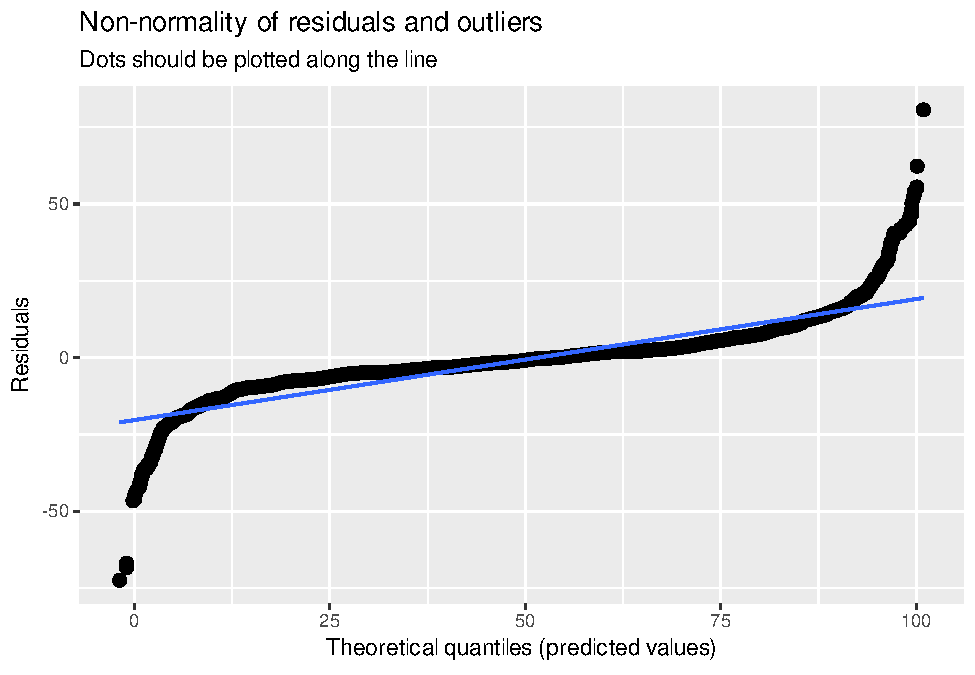
\includegraphics[width=0.25\linewidth]{OBIWAN_LIRA_files/figure-latex/unnamed-chunk-7-1} 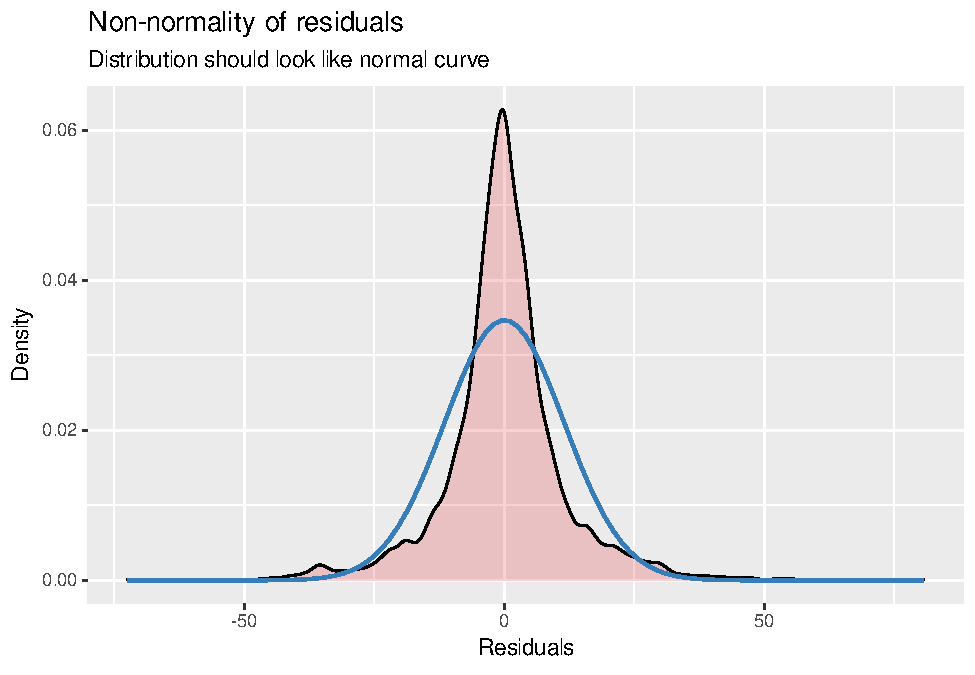
\includegraphics[width=0.25\linewidth]{OBIWAN_LIRA_files/figure-latex/unnamed-chunk-7-2} 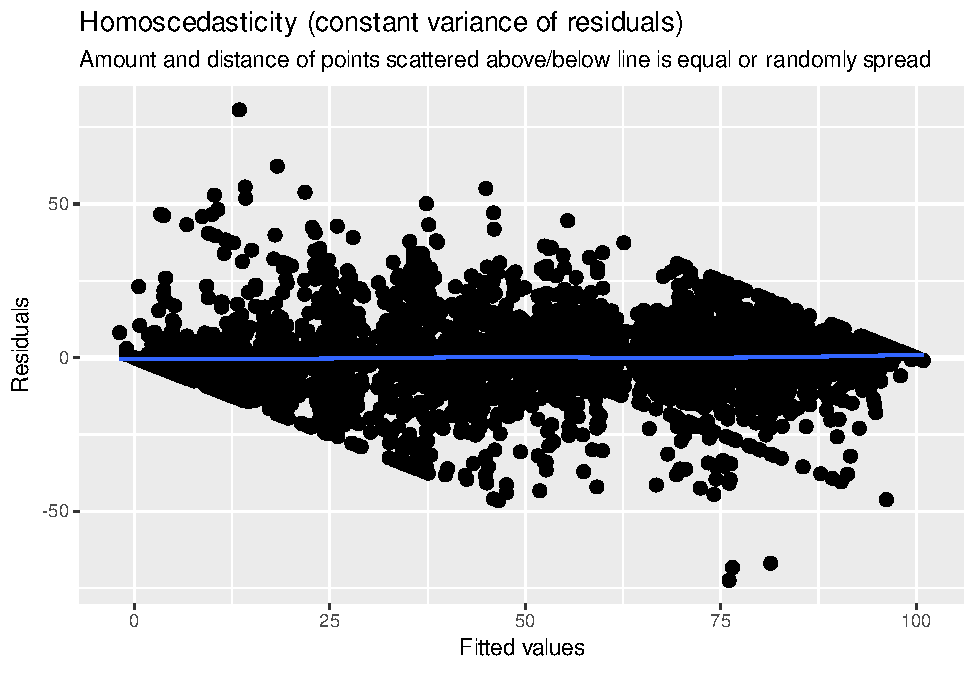
\includegraphics[width=0.25\linewidth]{OBIWAN_LIRA_files/figure-latex/unnamed-chunk-7-3} 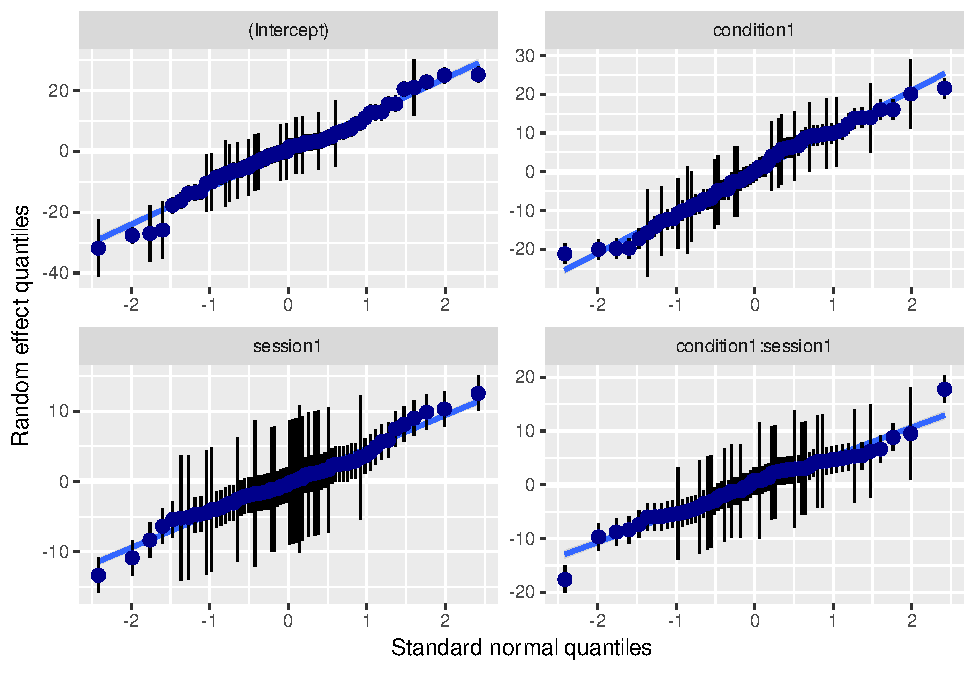
\includegraphics[width=0.25\linewidth]{OBIWAN_LIRA_files/figure-latex/unnamed-chunk-7-4} 

}

\caption{Model assumptions.}\label{fig:unnamed-chunk-7}
\end{figure}

\hfill\break
\hfill\break

\begin{figure}

{\centering 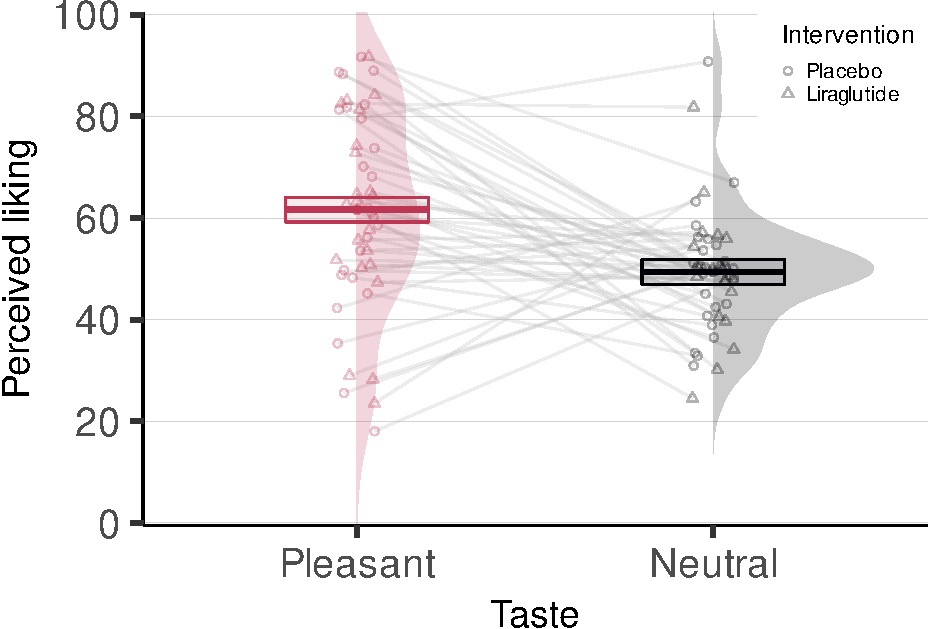
\includegraphics{OBIWAN_LIRA_files/figure-latex/HED_plot-1} 

}

\caption{Perceived liking (Taste) by solution.}\label{fig:HED_plot}
\end{figure}

\hfill\break
\hfill\break

\hypertarget{fmri-analysis}{%
\section{fMRI Analysis}\label{fmri-analysis}}

check out ``analysis\_LIRA\_fMRI.R'' for more details

Contrast Post \textgreater{} Pre in HF\\

\begin{Shaded}
\begin{Highlighting}[]
\NormalTok{res}\SpecialCharTok{$}\NormalTok{p.value }\OtherTok{=} \FunctionTok{as.numeric}\NormalTok{(res}\SpecialCharTok{$}\NormalTok{p.value)}
\NormalTok{res}\SpecialCharTok{$}\NormalTok{p.value }\OtherTok{=} \FunctionTok{ifelse}\NormalTok{(res}\SpecialCharTok{$}\NormalTok{p.value }\SpecialCharTok{\textless{}} \FloatTok{0.05}\NormalTok{,}\FunctionTok{paste}\NormalTok{(}\StringTok{"\textless{}span style=}\SpecialCharTok{\textbackslash{}"}\StringTok{ font{-}weight: bold; }\SpecialCharTok{\textbackslash{}"}\StringTok{ \textgreater{}"}\NormalTok{ ,}\FunctionTok{sprintf}\NormalTok{(}\StringTok{"\%.3f"}\NormalTok{,res}\SpecialCharTok{$}\NormalTok{p.value), }\StringTok{"\textless{}/span\textgreater{}"}\NormalTok{),  }\FunctionTok{paste}\NormalTok{(}\StringTok{"\textless{}span\textgreater{}"}\NormalTok{ ,}\FunctionTok{sprintf}\NormalTok{(}\StringTok{"\%.3f"}\NormalTok{,res}\SpecialCharTok{$}\NormalTok{p.value), }\StringTok{"\textless{}/span\textgreater{}"}\NormalTok{))}

\NormalTok{res}\SpecialCharTok{$}\NormalTok{F }\OtherTok{=} \FunctionTok{unlist}\NormalTok{(}\FunctionTok{str\_split}\NormalTok{(}\FunctionTok{gsub}\NormalTok{(}\StringTok{"[\^{}0{-}9.,{-}]"}\NormalTok{, }\StringTok{""}\NormalTok{, res}\SpecialCharTok{$}\NormalTok{F), }\StringTok{","}\NormalTok{));res}\SpecialCharTok{$}\NormalTok{pes }\OtherTok{=} \FunctionTok{unlist}\NormalTok{(}\FunctionTok{str\_split}\NormalTok{(}\FunctionTok{gsub}\NormalTok{(}\StringTok{"[\^{}0{-}9.,{-}]"}\NormalTok{, }\StringTok{""}\NormalTok{, res}\SpecialCharTok{$}\NormalTok{pes), }\StringTok{","}\NormalTok{));}
\NormalTok{res}\SpecialCharTok{$}\StringTok{\textasciigrave{}}\AttributeTok{90\% CI}\StringTok{\textasciigrave{}} \OtherTok{=} \FunctionTok{paste}\NormalTok{(}\FunctionTok{sprintf}\NormalTok{(}\StringTok{"\%.3f"}\NormalTok{,PES.hf[,}\DecValTok{2}\NormalTok{]), }\StringTok{"{-}"}\NormalTok{, }\FunctionTok{sprintf}\NormalTok{(}\StringTok{"\%.3f"}\NormalTok{,PES.hf[,}\DecValTok{3}\NormalTok{]))}

\NormalTok{res}\SpecialCharTok{$}\NormalTok{p.value[}\DecValTok{1}\NormalTok{]}\OtherTok{=} \StringTok{"\textless{}span style=}\SpecialCharTok{\textbackslash{}"}\StringTok{ font{-}weight: bold;    }\SpecialCharTok{\textbackslash{}"}\StringTok{ \textgreater{}\textbackslash{}u003C 0.001\textless{}/span\textgreater{}"}
\CommentTok{\#res$pes[c(5,7,8)]= c("\textbackslash{}u003C 0.001")}
\FunctionTok{colnames}\NormalTok{(res)[}\DecValTok{3}\SpecialCharTok{:}\DecValTok{5}\NormalTok{] }\OtherTok{=} \FunctionTok{c}\NormalTok{( }\FunctionTok{paste}\NormalTok{(}\StringTok{"F("}\NormalTok{, res}\SpecialCharTok{$}\NormalTok{df[}\DecValTok{1}\NormalTok{], }\StringTok{")"}\NormalTok{, }\AttributeTok{sep=}\StringTok{""}\NormalTok{),}\StringTok{"\&eta;\textless{}sub\textgreater{}p\textless{}/sub\textgreater{}\textless{}sup\textgreater{}2\textless{}/sup\textgreater{}"}\NormalTok{, }\StringTok{"p"}\NormalTok{)}
\NormalTok{res[}\FunctionTok{c}\NormalTok{(}\DecValTok{1}\NormalTok{,}\DecValTok{4}\NormalTok{,}\DecValTok{6}\NormalTok{,}\DecValTok{3}\NormalTok{,}\DecValTok{5}\NormalTok{)]  }\SpecialCharTok{\%\textgreater{}\%} \FunctionTok{kbl}\NormalTok{(}\AttributeTok{digits =} \DecValTok{2}\NormalTok{, }\AttributeTok{escape =}\NormalTok{ F,}\AttributeTok{row.names =}\NormalTok{ F)  }\SpecialCharTok{\%\textgreater{}\%}
  \FunctionTok{kable\_styling}\NormalTok{(}\AttributeTok{latex\_options =} \StringTok{"striped"}\NormalTok{, }\AttributeTok{position =} \StringTok{"center"}\NormalTok{, }\AttributeTok{full\_width =}\NormalTok{ F) }
\end{Highlighting}
\end{Shaded}

\begin{table}[H]
\centering
\begin{tabular}[t]{l|l|l|l|l}
\hline
Effect & &eta;<sub>p</sub><sup>2</sup> & 90% CI & F(1, 38) & p\\
\hline
\cellcolor{gray!6}{intervention} & \cellcolor{gray!6}{.345} & \cellcolor{gray!6}{0.145 - 0.498} & \cellcolor{gray!6}{20.01} & \cellcolor{gray!6}{<span style=" font-weight: bold;    " >< 0.001</span>}\\
\hline
BMI_diff & .119 & 0.007 - 0.281 & 5.14 & <span style=" font-weight: bold; " > 0.029 </span>\\
\hline
\cellcolor{gray!6}{age} & \cellcolor{gray!6}{.171} & \cellcolor{gray!6}{0.027 - 0.337} & \cellcolor{gray!6}{7.84} & \cellcolor{gray!6}{<span style=" font-weight: bold; " > 0.008 </span>}\\
\hline
\end{tabular}
\end{table}

\begin{Shaded}
\begin{Highlighting}[]
\CommentTok{\#print(\textquotesingle{}PES: intervention: Overall higher weight loss for treament (Liraglutide) group\textquotesingle{})}
\CommentTok{\#PES.weight[1,]}
\end{Highlighting}
\end{Shaded}

\begin{figure}

{\centering 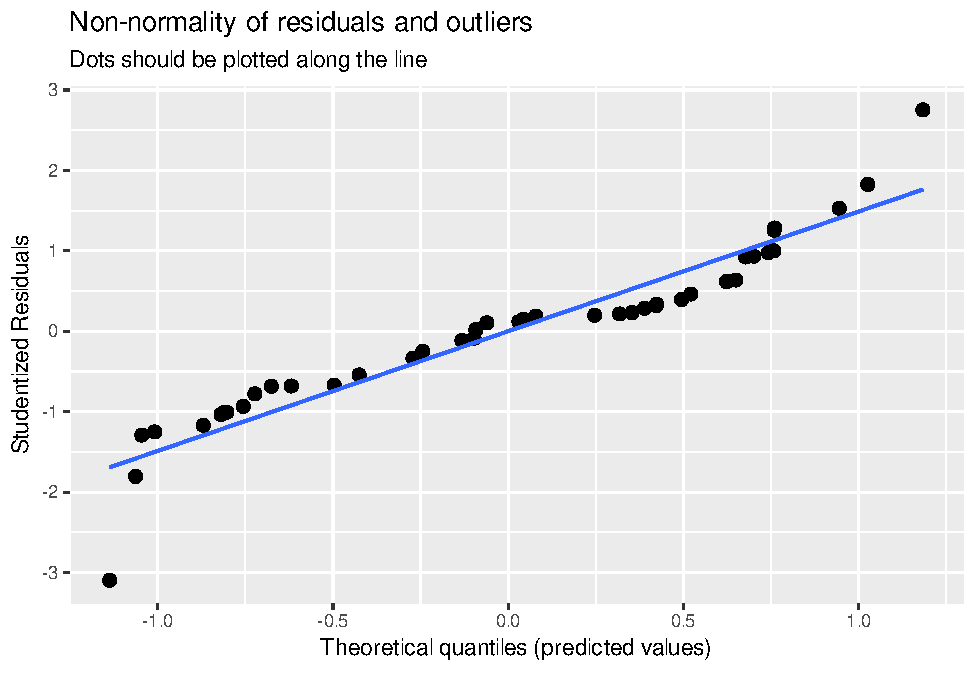
\includegraphics[width=0.25\linewidth]{OBIWAN_LIRA_files/figure-latex/unnamed-chunk-8-1} 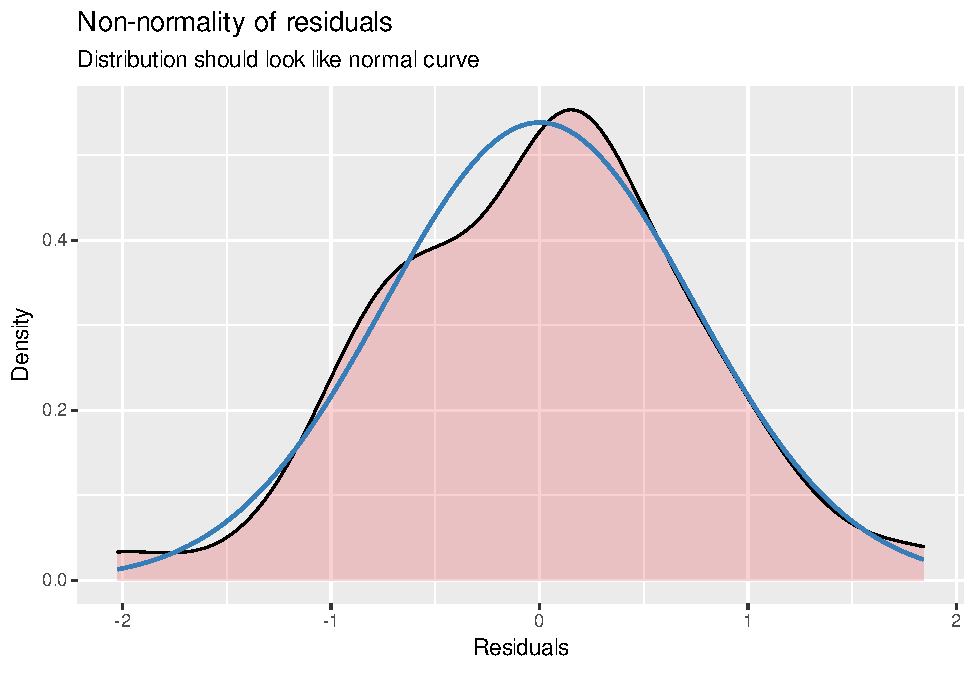
\includegraphics[width=0.25\linewidth]{OBIWAN_LIRA_files/figure-latex/unnamed-chunk-8-2} 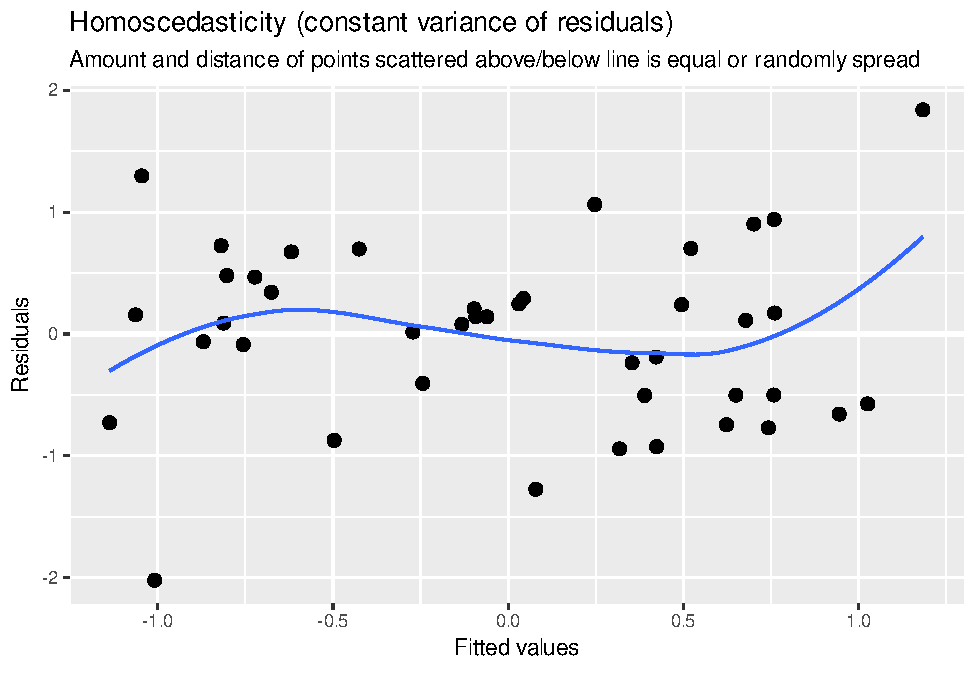
\includegraphics[width=0.25\linewidth]{OBIWAN_LIRA_files/figure-latex/unnamed-chunk-8-3} 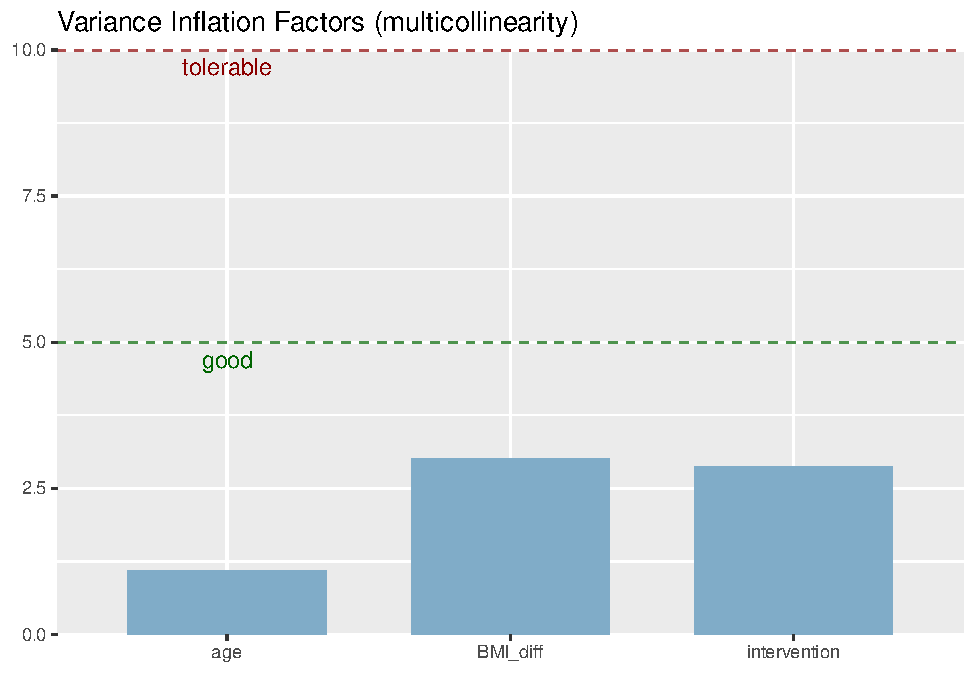
\includegraphics[width=0.25\linewidth]{OBIWAN_LIRA_files/figure-latex/unnamed-chunk-8-4} 

}

\caption{Model assumptions.}\label{fig:unnamed-chunk-8}
\end{figure}

\hfill\break
\hfill\break

\begin{figure}

\hfill{}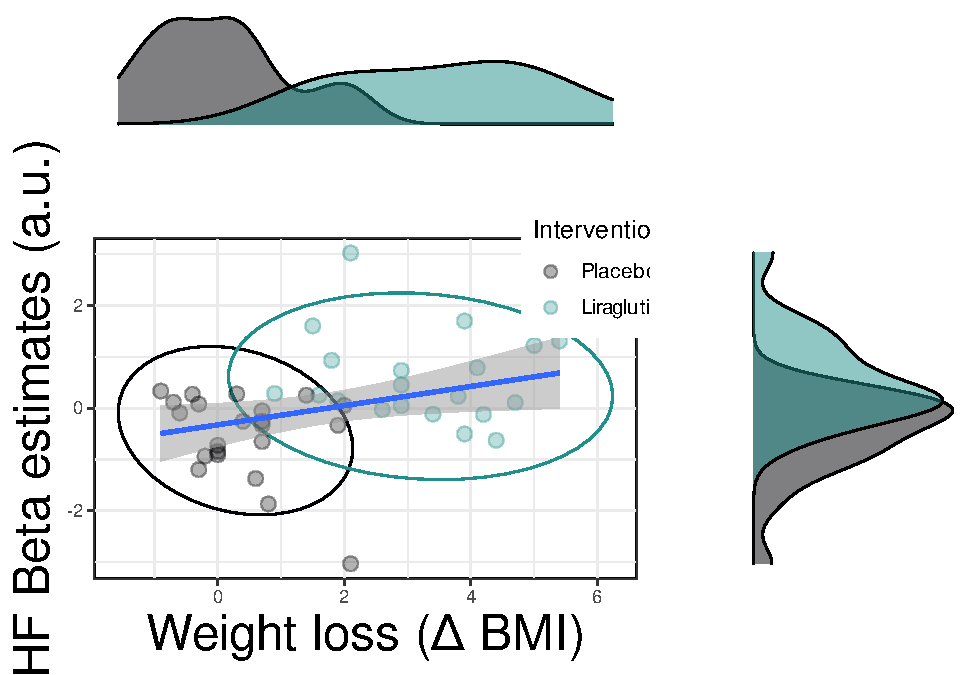
\includegraphics{OBIWAN_LIRA_files/figure-latex/HED_fmri_plot-1} 

\caption{Beta estimates from hippocampal formation during Hedonic reactivity test (Post > Pre) by intervention and correlation with weight loss.}\label{fig:HED_fmri_plot}
\end{figure}

\hfill\break

\begin{table}[H]

\caption{\label{tab:hpp_mediate_res}Mediation Analysis: DV = Weight loss, IV = HF activity during reward consumption}
\centering
\begin{tabular}[t]{l|l|l|l}
\hline
 & Estimates & 95% CI & p\\
\hline
Indirect effect mediated through HF & -0.484 & (-1.034, -0.045) & <span style=" font-weight: bold; " > 0.032 </span>\\
\hline
Direct effect & 3.226 & (2.512, 3.943) & <span style=" font-weight: bold; " > < 0.001 <span>\\
\hline
Total effect & 2.742 & (2.073, 3.348) & <span style=" font-weight: bold; " > < 0.001 <span>\\
\hline
Proportion of effect mediated through HF & -0.170 &  & \\
\hline
\end{tabular}
\end{table}

\begin{Shaded}
\begin{Highlighting}[]
\FunctionTok{par}\NormalTok{(}\AttributeTok{mar=}\FunctionTok{c}\NormalTok{(}\DecValTok{0}\NormalTok{,}\DecValTok{0}\NormalTok{,}\DecValTok{0}\NormalTok{,}\DecValTok{0}\NormalTok{)); psych}\SpecialCharTok{::}\FunctionTok{mediate.diagram}\NormalTok{(medi, }\AttributeTok{show.c =}\NormalTok{ F, }\AttributeTok{main=} \StringTok{""}\NormalTok{, }\AttributeTok{ylim=}\FunctionTok{c}\NormalTok{(}\FloatTok{4.5}\NormalTok{,}\FloatTok{7.3}\NormalTok{))}
\FunctionTok{text}\NormalTok{(}\DecValTok{3}\NormalTok{, }\FloatTok{6.5}\NormalTok{, }\StringTok{"A ***"}\NormalTok{,  }\AttributeTok{cex =}\NormalTok{ .}\DecValTok{8}\NormalTok{); }\FunctionTok{text}\NormalTok{(}\DecValTok{7}\NormalTok{, }\FloatTok{6.5}\NormalTok{, }\StringTok{"B *"}\NormalTok{,  }\AttributeTok{cex =}\NormalTok{ .}\DecValTok{8}\NormalTok{);  }\FunctionTok{text}\NormalTok{(}\FloatTok{5.8}\NormalTok{, }\FloatTok{4.9}\NormalTok{, }\StringTok{"***"}\NormalTok{,  }\AttributeTok{cex =}\NormalTok{ .}\DecValTok{8}\NormalTok{); }\FunctionTok{text}\NormalTok{(}\DecValTok{5}\NormalTok{, }\FloatTok{6.7}\NormalTok{, }\StringTok{"AB *"}\NormalTok{,  }\AttributeTok{cex =}\NormalTok{ .}\DecValTok{8}\NormalTok{)}
\end{Highlighting}
\end{Shaded}

\begin{figure}

{\centering 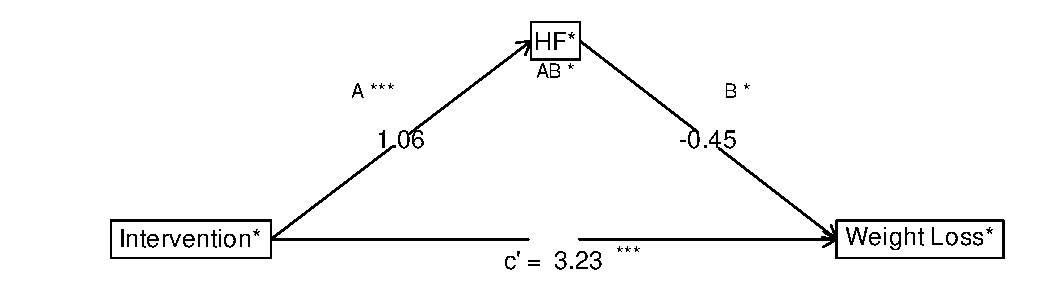
\includegraphics{OBIWAN_LIRA_files/figure-latex/unnamed-chunk-9-1} 

}

\caption{Mediation path.}\label{fig:unnamed-chunk-9}
\end{figure}

\hfill\break

\begin{figure}

\hfill{}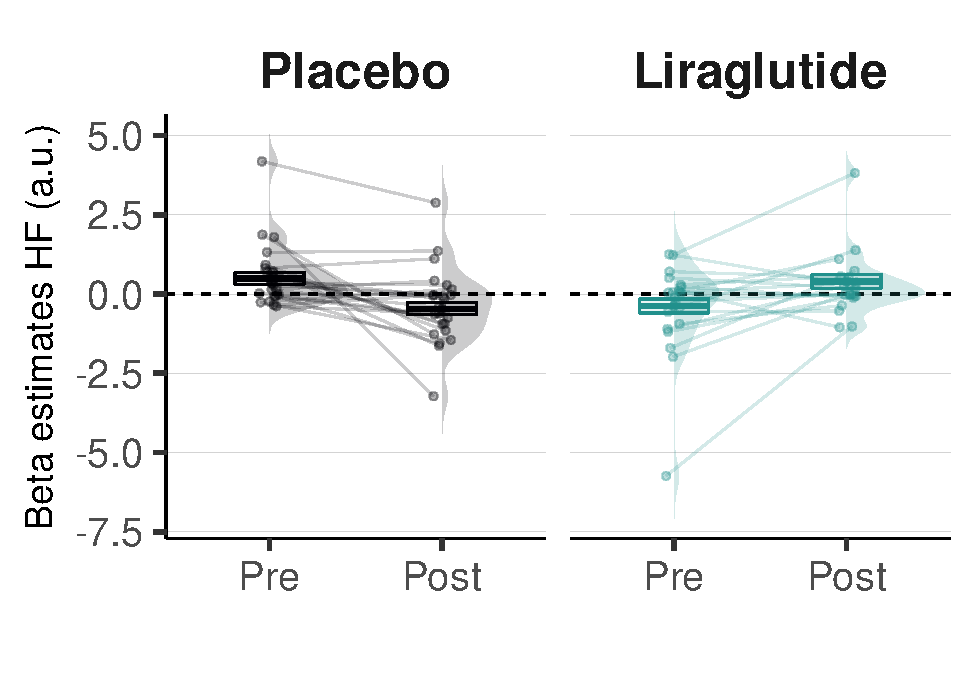
\includegraphics{OBIWAN_LIRA_files/figure-latex/HED_fmri_plot_HF-1} 

\caption{Beta estimates from hippocampal formation during Hedonic reactivity testby session by intervention.}\label{fig:HED_fmri_plot_HF}
\end{figure}

\begin{Shaded}
\begin{Highlighting}[]
\FunctionTok{cairo\_pdf}\NormalTok{(}\StringTok{\textquotesingle{}figures/Figure\_HED\_fmri\_HF.pdf\textquotesingle{}}\NormalTok{)}
\FunctionTok{print}\NormalTok{(ppp)}
\FunctionTok{dev.off}\NormalTok{()}
\end{Highlighting}
\end{Shaded}

\begin{verbatim}
## cairo_pdf 
##         2
\end{verbatim}

\begin{figure}

\hfill{}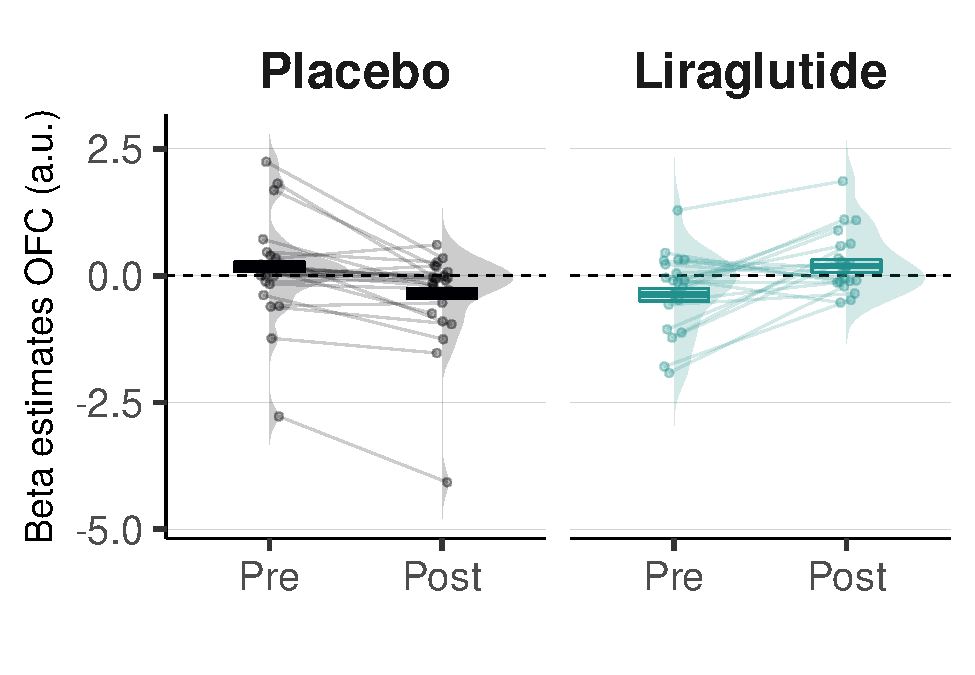
\includegraphics{OBIWAN_LIRA_files/figure-latex/HED_fmri_plot_OFC-1} 

\caption{Beta estimates from OFC during Hedonic reactivity test by session by intervention.}\label{fig:HED_fmri_plot_OFC}
\end{figure}

\begin{Shaded}
\begin{Highlighting}[]
\FunctionTok{cairo\_pdf}\NormalTok{(}\StringTok{\textquotesingle{}figures/Figure\_HED\_fmri\_OFC.pdf\textquotesingle{}}\NormalTok{)}
\FunctionTok{print}\NormalTok{(ppp)}
\FunctionTok{dev.off}\NormalTok{()}
\end{Highlighting}
\end{Shaded}

\begin{verbatim}
## cairo_pdf 
##         2
\end{verbatim}

\end{document}
